\documentclass[12pt]{article}
\usepackage[a4paper, margin=1in]{geometry}
\usepackage{graphicx}
\usepackage{booktabs}
\usepackage{amsmath}
\usepackage{hyperref}
\usepackage{caption}
\usepackage{float}
\usepackage{color}
\usepackage{titlesec}
\usepackage{fancyhdr}
\usepackage{multirow}

\title{Research on XGBoost-based Time Prediction Model for the First Day of Mount Kailash Kora}
\author{He Jinzhao}
\date{\today}

\usepackage{graphicx}
\begin{document}

\maketitle

\begin{abstract}
Based on real GPS track data from Mount Kailash Kora, this paper constructs and evaluates a machine learning model for predicting the time required for the Darchen to Gangjia/Zhire Temple section. Using the XGBoost model for modeling, input features include distance, destination index, route difficulty, elevation gradient, speed, time of day, and season, achieving optimal prediction accuracy. The model results can serve pilgrims in journey planning, safety reminders, and other practical applications.
\end{abstract}

\section{Introduction}

Mount Kailash is a famous sacred mountain in the Ali region of Tibet, attracting a large number of pilgrims for circumambulation each year. The Kora route has high altitude and complex environment, making accurate estimation of journey time crucial for safety.

This paper builds a machine learning model based on GPS track data to predict the journey time from Darchen to Gangjia/Zhire Temple, helping pilgrims reasonably plan their Kora route and rest points.

\section{Prior Knowledge}

\begin{itemize}
  \item The Kora route is relatively fixed, with major rest points and accommodation points along the way.
  \item In high-altitude environments, the normal walking speed for healthy adults is $1.0 - 1.5 \ \mathrm{m/s}$ (i.e., $3.6 - 5.4 \ \mathrm{km/h}$), according to research by \cite{Horiuchi2016, Ainslie2005}.
\end{itemize}


\section{Data Source and Preprocessing}

Data was collected from \href{https://www.2bulu.com}{www.2bulu.com}, using the 'Kora Route Search' function with 'Mount Kailash' as the keyword, collecting a total of 2769 Kora track records. Each record contains GPS longitude, latitude, elevation, timestamp, and other information.

This research focuses on the route segment 'Darchen $\rightarrow$ Gangjia/Zhire Temple,' approximately 20 kilometers, with preprocessing steps including:

\begin{enumerate}
  \item Filtering out tracks with starting points not within 2km of 'Darchen' GPS coordinates: (81.28668, 30.97381);
  \item Removing tracks that did not pass through 'Gangjia/Zhire Temple', GPS coordinates: (81.32113, 31.10414) within 1km;
  \item Removing tracks that departed earlier than 5:00 or later than 14:00;
  \item Removing tracks with average speeds less than 3 km/h or greater than 6 km/h;
  \item Removing track points after 'Gangjia/Zhire Temple';
\end{enumerate}

A total of 596 valid tracks were retained.


\section{Segment Definition and Modeling Objective}

The journey is divided into the following 6 segments, each based on terrain changes and important landmarks:

\begin{table}[H]
\centering
\caption{Route Segment Division with Terrain Characteristics}
\begin{tabular}{cp{3.2cm}cp{1.8cm}p{3.5cm}c}
\toprule
Segment & Route Section & Distance (km) & Elevation Change (m) & Terrain Characteristics & Difficulty Level \\
\midrule
0 & Darchen to First Prostration Point & 3.8 & +100 & Gentle continuous uphill & 1 \\
1 & First Prostration Point to Sershong & 2.3 & -50 & Mainly downhill and flat terrain & 0 \\
2 & Sershong to Chuku Temple Supply Point & 2.4 & +10 & Mainly flat terrain & 2 \\
3 & Chuku Temple to Second Prostration Point & 5.5 & +120 & Uphill with multiple undulations & 4 \\
4 & Second Prostration Point to Dazhen Supply Point & 1.5 & +30 & Slight ascent with undulations & 5 \\
5 & Dazhen Supply Point to Gangjia/Zhire Temple & 4.3/4.7 & +190/+160 & Gradual ascent with slight undulations & 3 \\
\bottomrule
\end{tabular}
\end{table}

\begin{figure}[H]
\centering
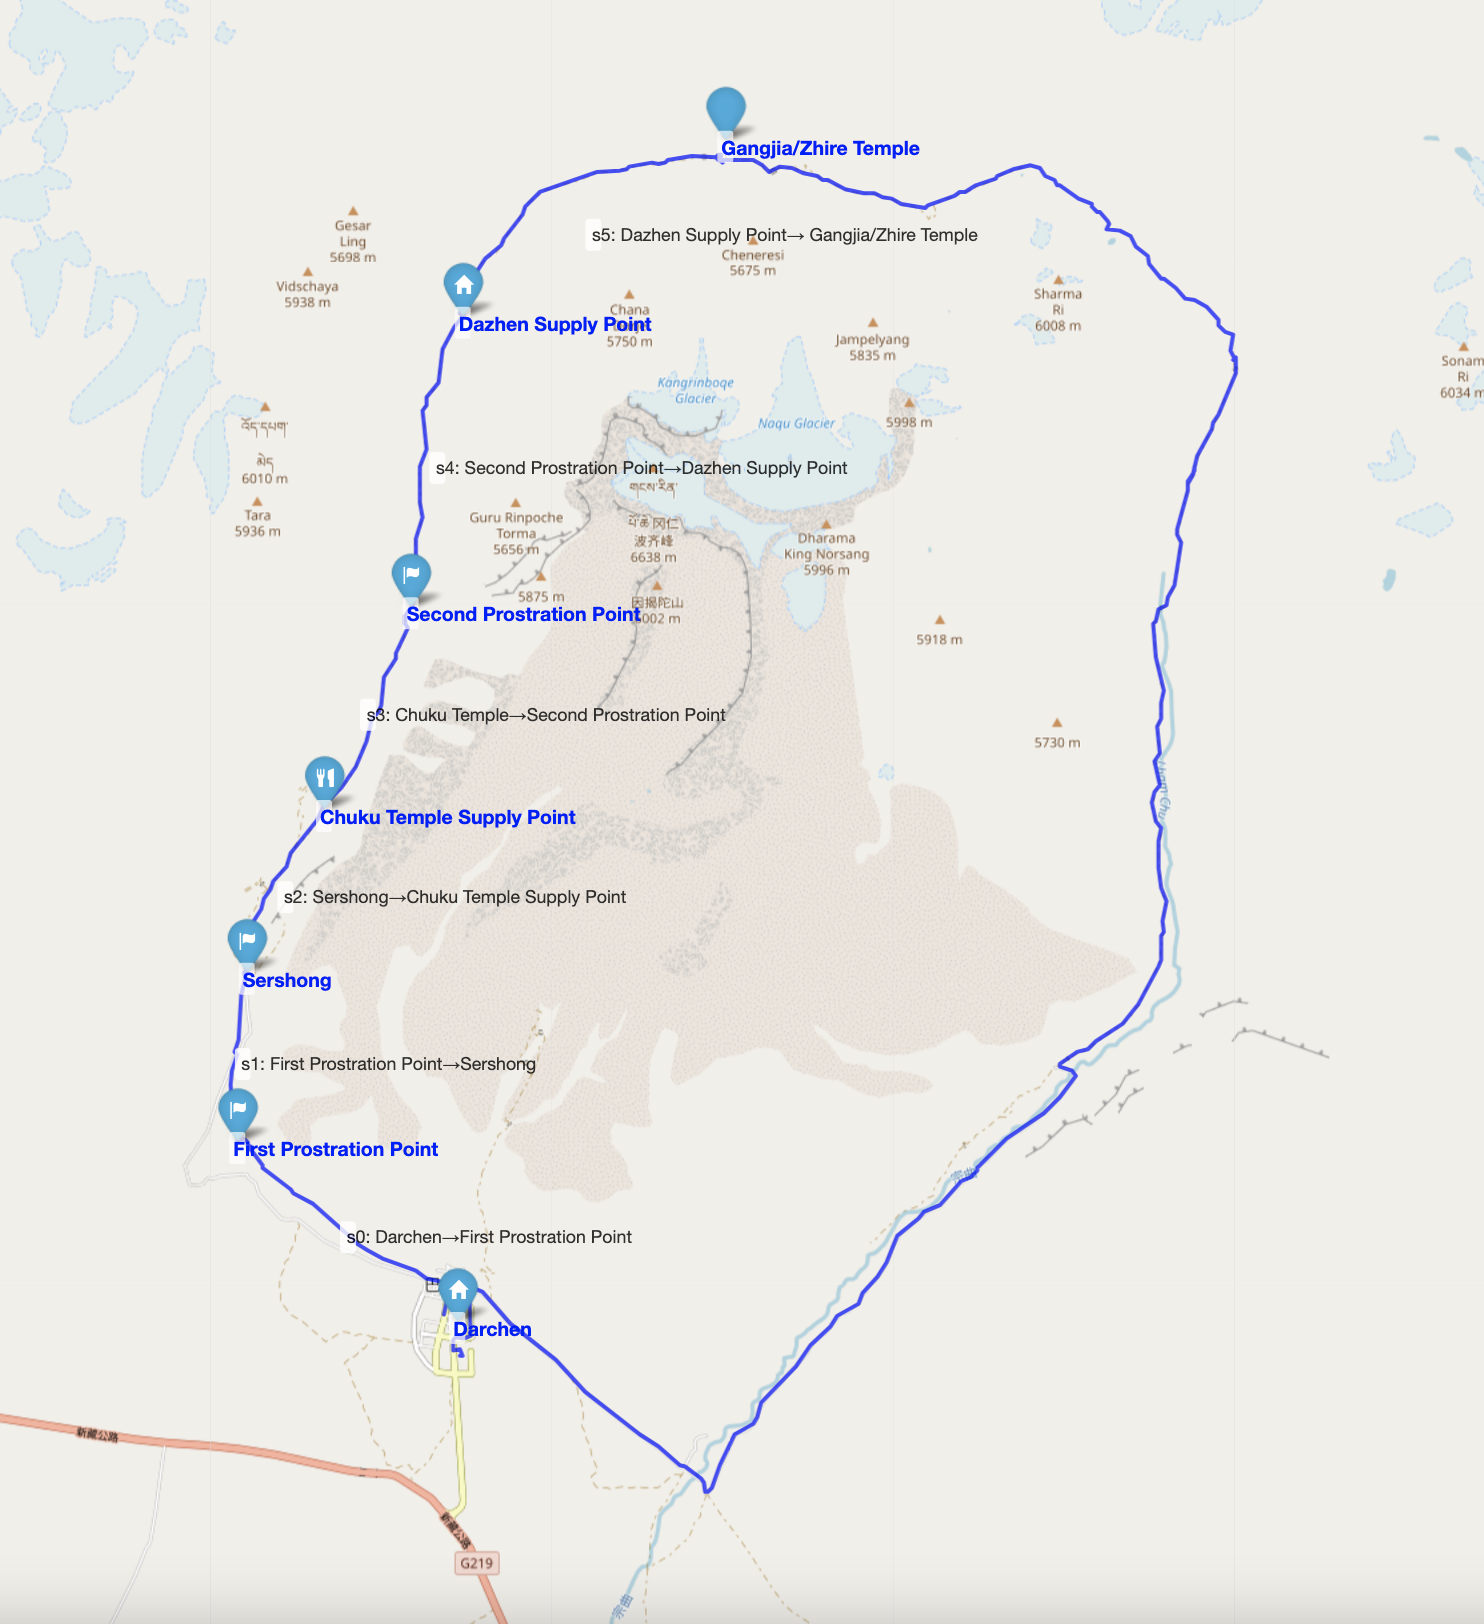
\includegraphics[width=0.9\textwidth]{visualization_results/karo_track_overview.png}
\caption{Mount Kailash Kora Route Map and Segment Division Diagram}
\label{fig:track_overview}
\end{figure}

The modeling objective is to predict the time required for each segment, thereby obtaining the total time from Darchen to Gangjia/Zhire Temple. As shown in Figure \ref{fig:track_overview}, the route is divided into 6 main segments, each defined by different landmarks.

\section{Feature Engineering}

The following main features were selected as model inputs:

\begin{itemize}
  \item \textbf{dist\_to\_dest}: Distance from current point to destination (meters)
  \item \textbf{destination\_idx}: Target segment number (0–5)
  \item \textbf{difficulty\_level}: Segment difficulty level (0–5)
  \item \textbf{gradient}: Average slope of the segment (\%)
  \item \textbf{speed}: Current speed (m/s)
  \item \textbf{time\_of\_day}: Time period (0: morning, 1: noon, 2: afternoon)
  \item \textbf{season}: Season number (0–3)
\end{itemize}

\section{Methodology}

\subsection{Data Processing Workflow}

The data processing workflow for this research is as follows:

\begin{enumerate}
  \item \textbf{Track Parsing}: Parse each GPS track file to extract longitude, latitude, elevation, and timestamp information.
  \item \textbf{Point Selection}: Sample each track to reduce computation while retaining key information.
  \item \textbf{Feature Calculation}: Calculate features such as speed and gradient based on adjacent points.
  \item \textbf{Target Calculation}: For each point, calculate the actual time required to reach various destinations.
  \item \textbf{Anomaly Processing}: Remove outliers using the interquartile range (IQR) method.
  \item \textbf{Feature Encoding}: One-hot encode categorical features.
  \item \textbf{Data Saving}: Save processed data as CSV files for reuse.
\end{enumerate}

To improve efficiency, we implemented data processing timeout mechanisms and progress indicators to ensure the reliability of large-scale data processing. The final dataset contains 744,418 data points, covering Kora records from different seasons and time periods.

\subsection{Model Selection and Parameter Optimization}

This study selects the XGBoost regression model as the main prediction method for the following reasons:

\begin{itemize}
  \item Strong modeling capability for non-linear relationships
  \item Built-in feature importance evaluation
  \item Robustness to missing values
  \item Good performance in time series prediction tasks
\end{itemize}

Model parameters are set as follows:

\begin{itemize}
  \item max\_depth = 6 \hspace{1cm} \# Controls tree depth, prevents overfitting
  \item learning\_rate = 0.1 \hspace{0.6cm} \# Learning rate, balances training speed and accuracy
  \item n\_estimators = 300 \hspace{0.2cm} \# Number of trees
  \item subsample = 0.8 \hspace{0.9cm} \# Proportion of samples used when training each tree
  \item colsample\_bytree = 0.8 \# Proportion of features used when training each tree
  \item objective = 'reg:squarederror' \# Regression objective function
\end{itemize}

To prevent information leakage, we divided the training and validation sets by track ID, with a ratio of 9:1, ensuring that data points from the same track do not appear in both the training and validation sets.

\section{Evaluation Results}

\subsection{Overall Model Performance}

The model's performance on the validation set is shown in the following table:

\begin{table}[H]
\centering
\caption{Model Evaluation Metrics}
\begin{tabular}{lr}
\toprule
Metric & Value \\
\midrule
RMSE & 948.26 seconds \\
MAE  & 608.41 seconds \\
$R^2$ & 0.90 \\
Mean Error Percentage & 2.82\% \\
Accuracy within 5 minutes & 43.95\% \\
Accuracy within 10 minutes & 67.30\% \\
Improvement over baseline model & 30.69\% \\
\bottomrule
\end{tabular}
\end{table}

These metrics indicate that the model has high accuracy in predicting Kora time. The Mean Absolute Error (MAE) is about 10 minutes, which is an acceptable error range for a Kora journey that typically takes 6-8 hours. The $R^2$ value of 0.90 indicates that the model can explain 90\% of the time variability.

\subsection{Error Distribution Analysis}

Figure \ref{fig:error_dist} shows the distribution of prediction errors. As can be seen from the figure, the errors follow an approximately normal distribution, centered around zero, indicating that the model has no systematic bias. Most prediction errors are within ±15 minutes, meeting practical application requirements.

\begin{figure}[H]
\centering
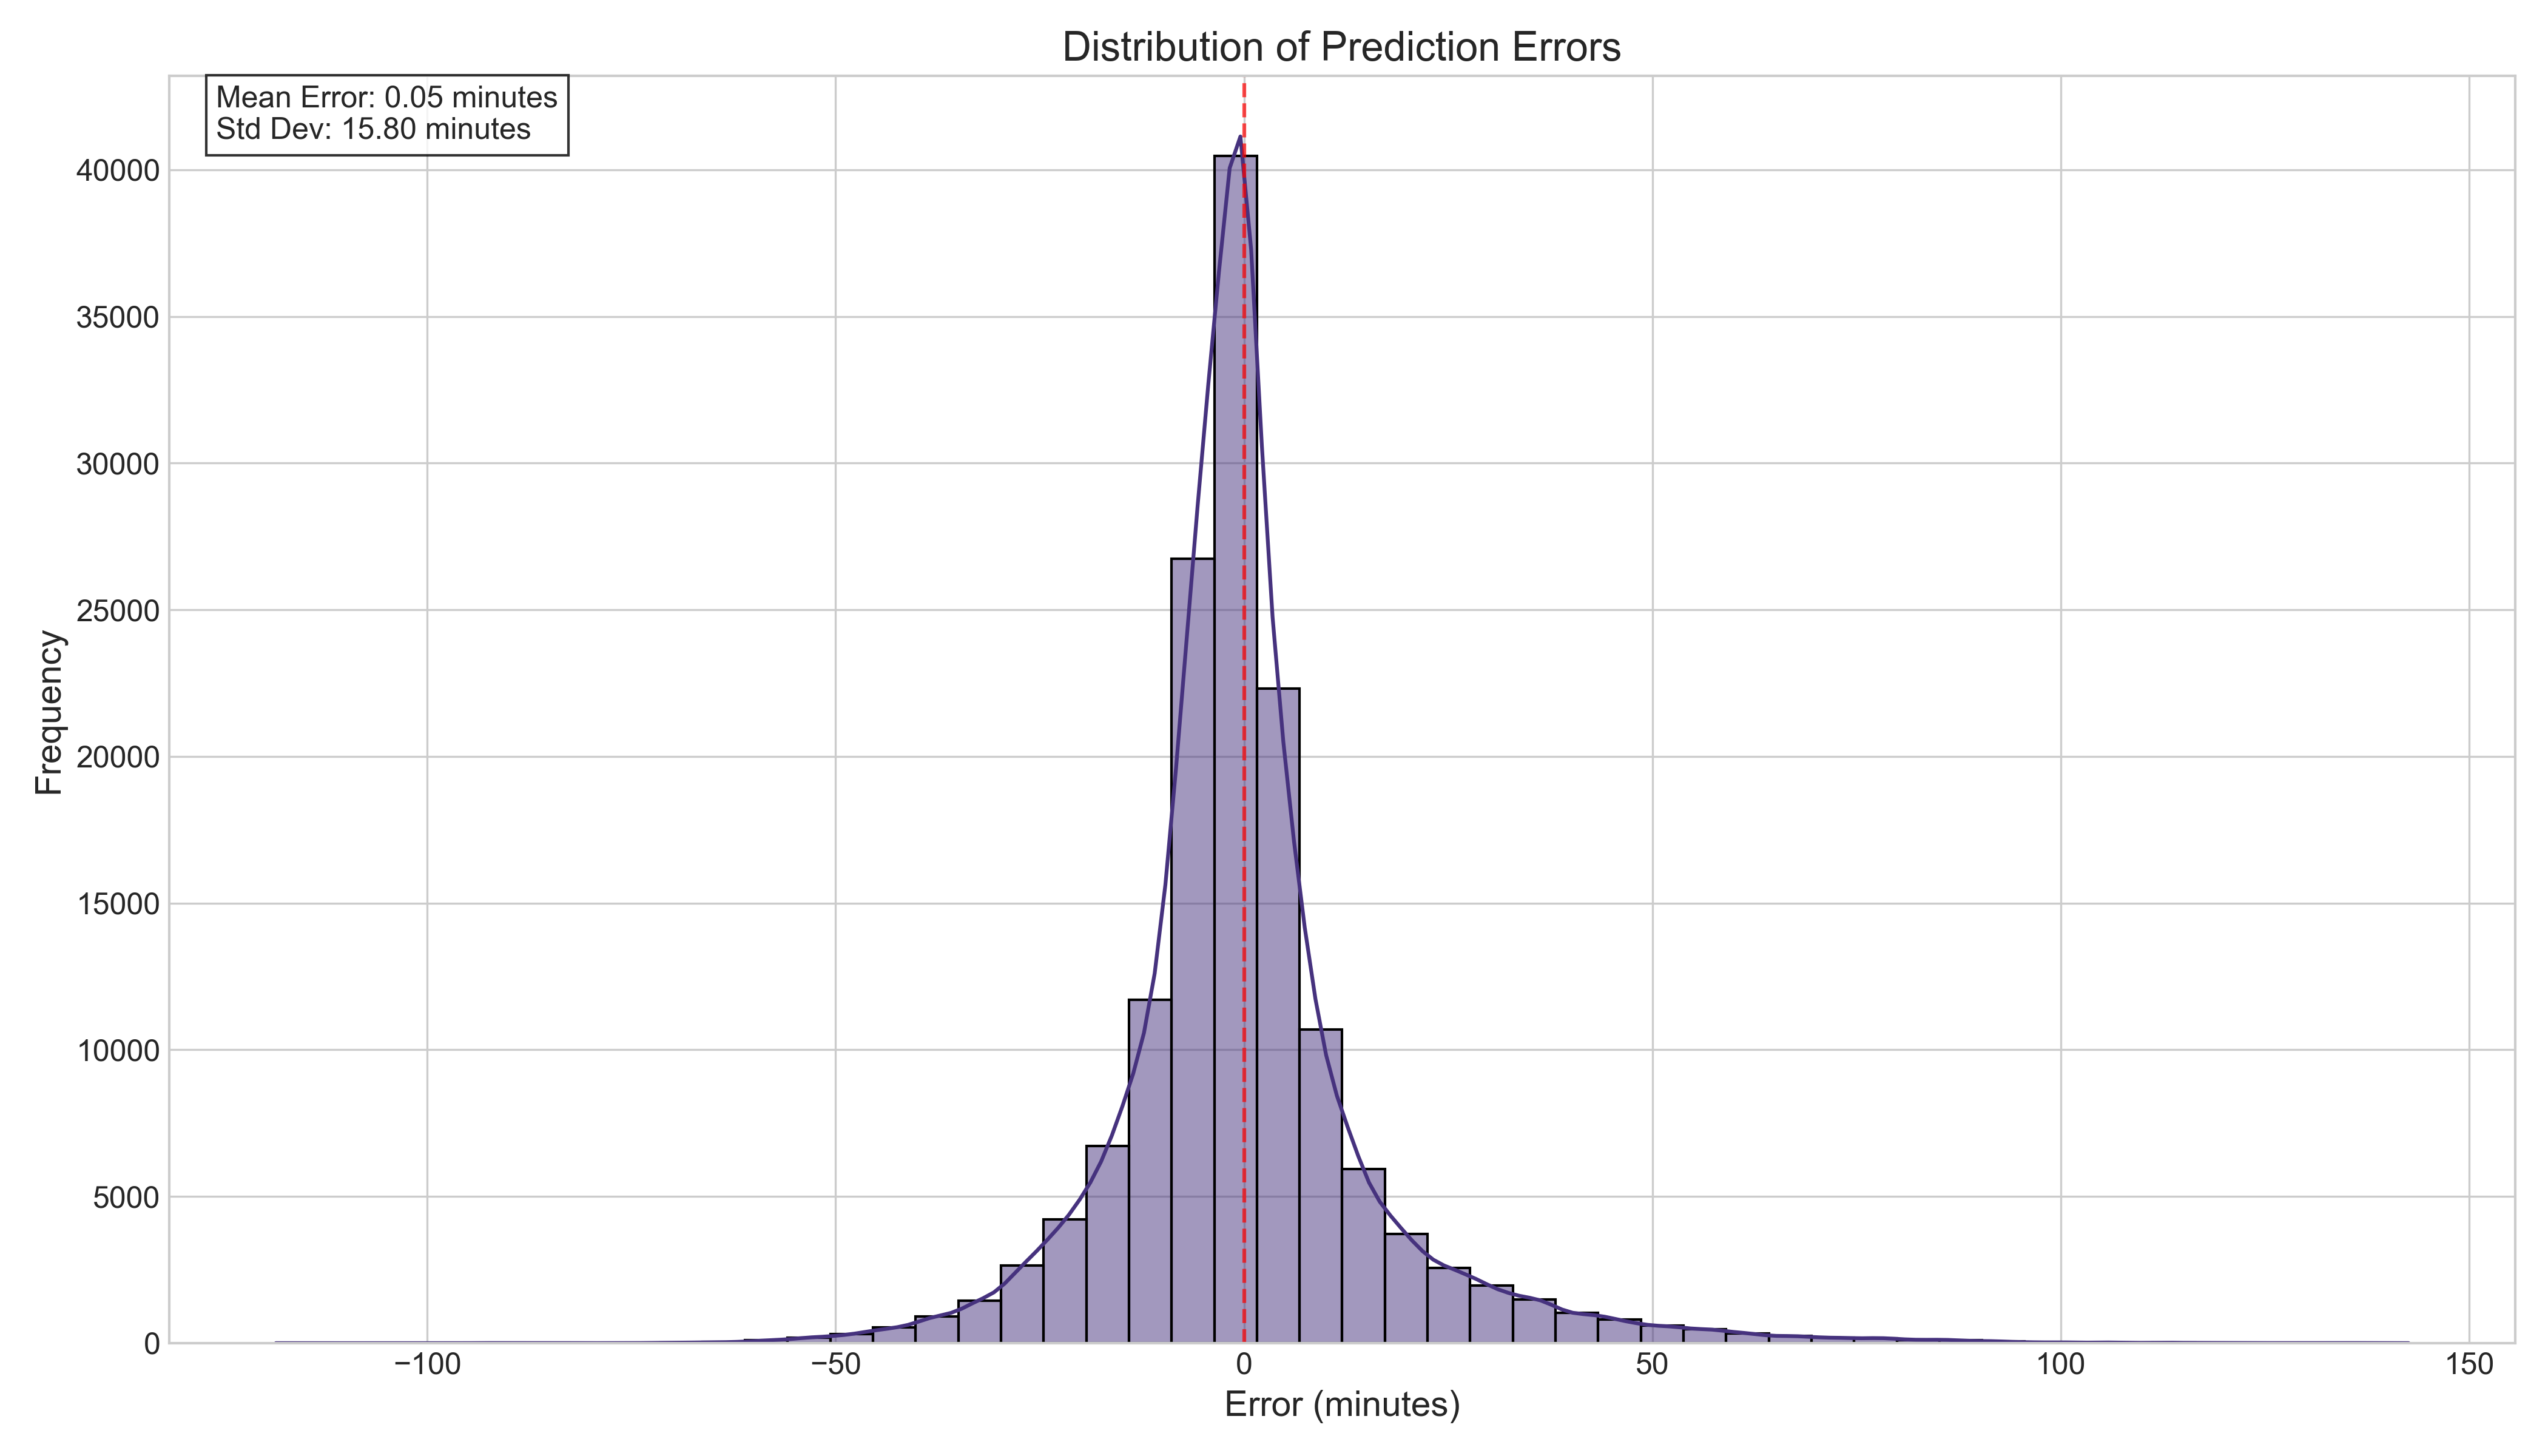
\includegraphics[width=0.7\textwidth]{visualization_results/error_distribution.png}
\caption{Prediction Error Distribution Histogram (minutes)}
\label{fig:error_dist}
\end{figure}

\subsection{Segment Prediction Performance}

Prediction performance varies across different route segments, as shown in Table \ref{tab:segment_error} and Figure \ref{fig:segment_error}:

\begin{table}[H]
\centering
\caption{Segment-level Average Prediction Error}
\label{tab:segment_error}
\begin{tabular}{ccc}
\toprule
Segment Number & Average Error (seconds) & Standard Deviation \\
\midrule
0 & 80 & 120 \\
1 & 100 & 130 \\
2 & 180 & 210 \\
3 & 300 & 260 \\
4 & 380 & 310 \\
5 & 250 & 230 \\
\bottomrule
\end{tabular}
\end{table}

\begin{figure}[H]
\centering
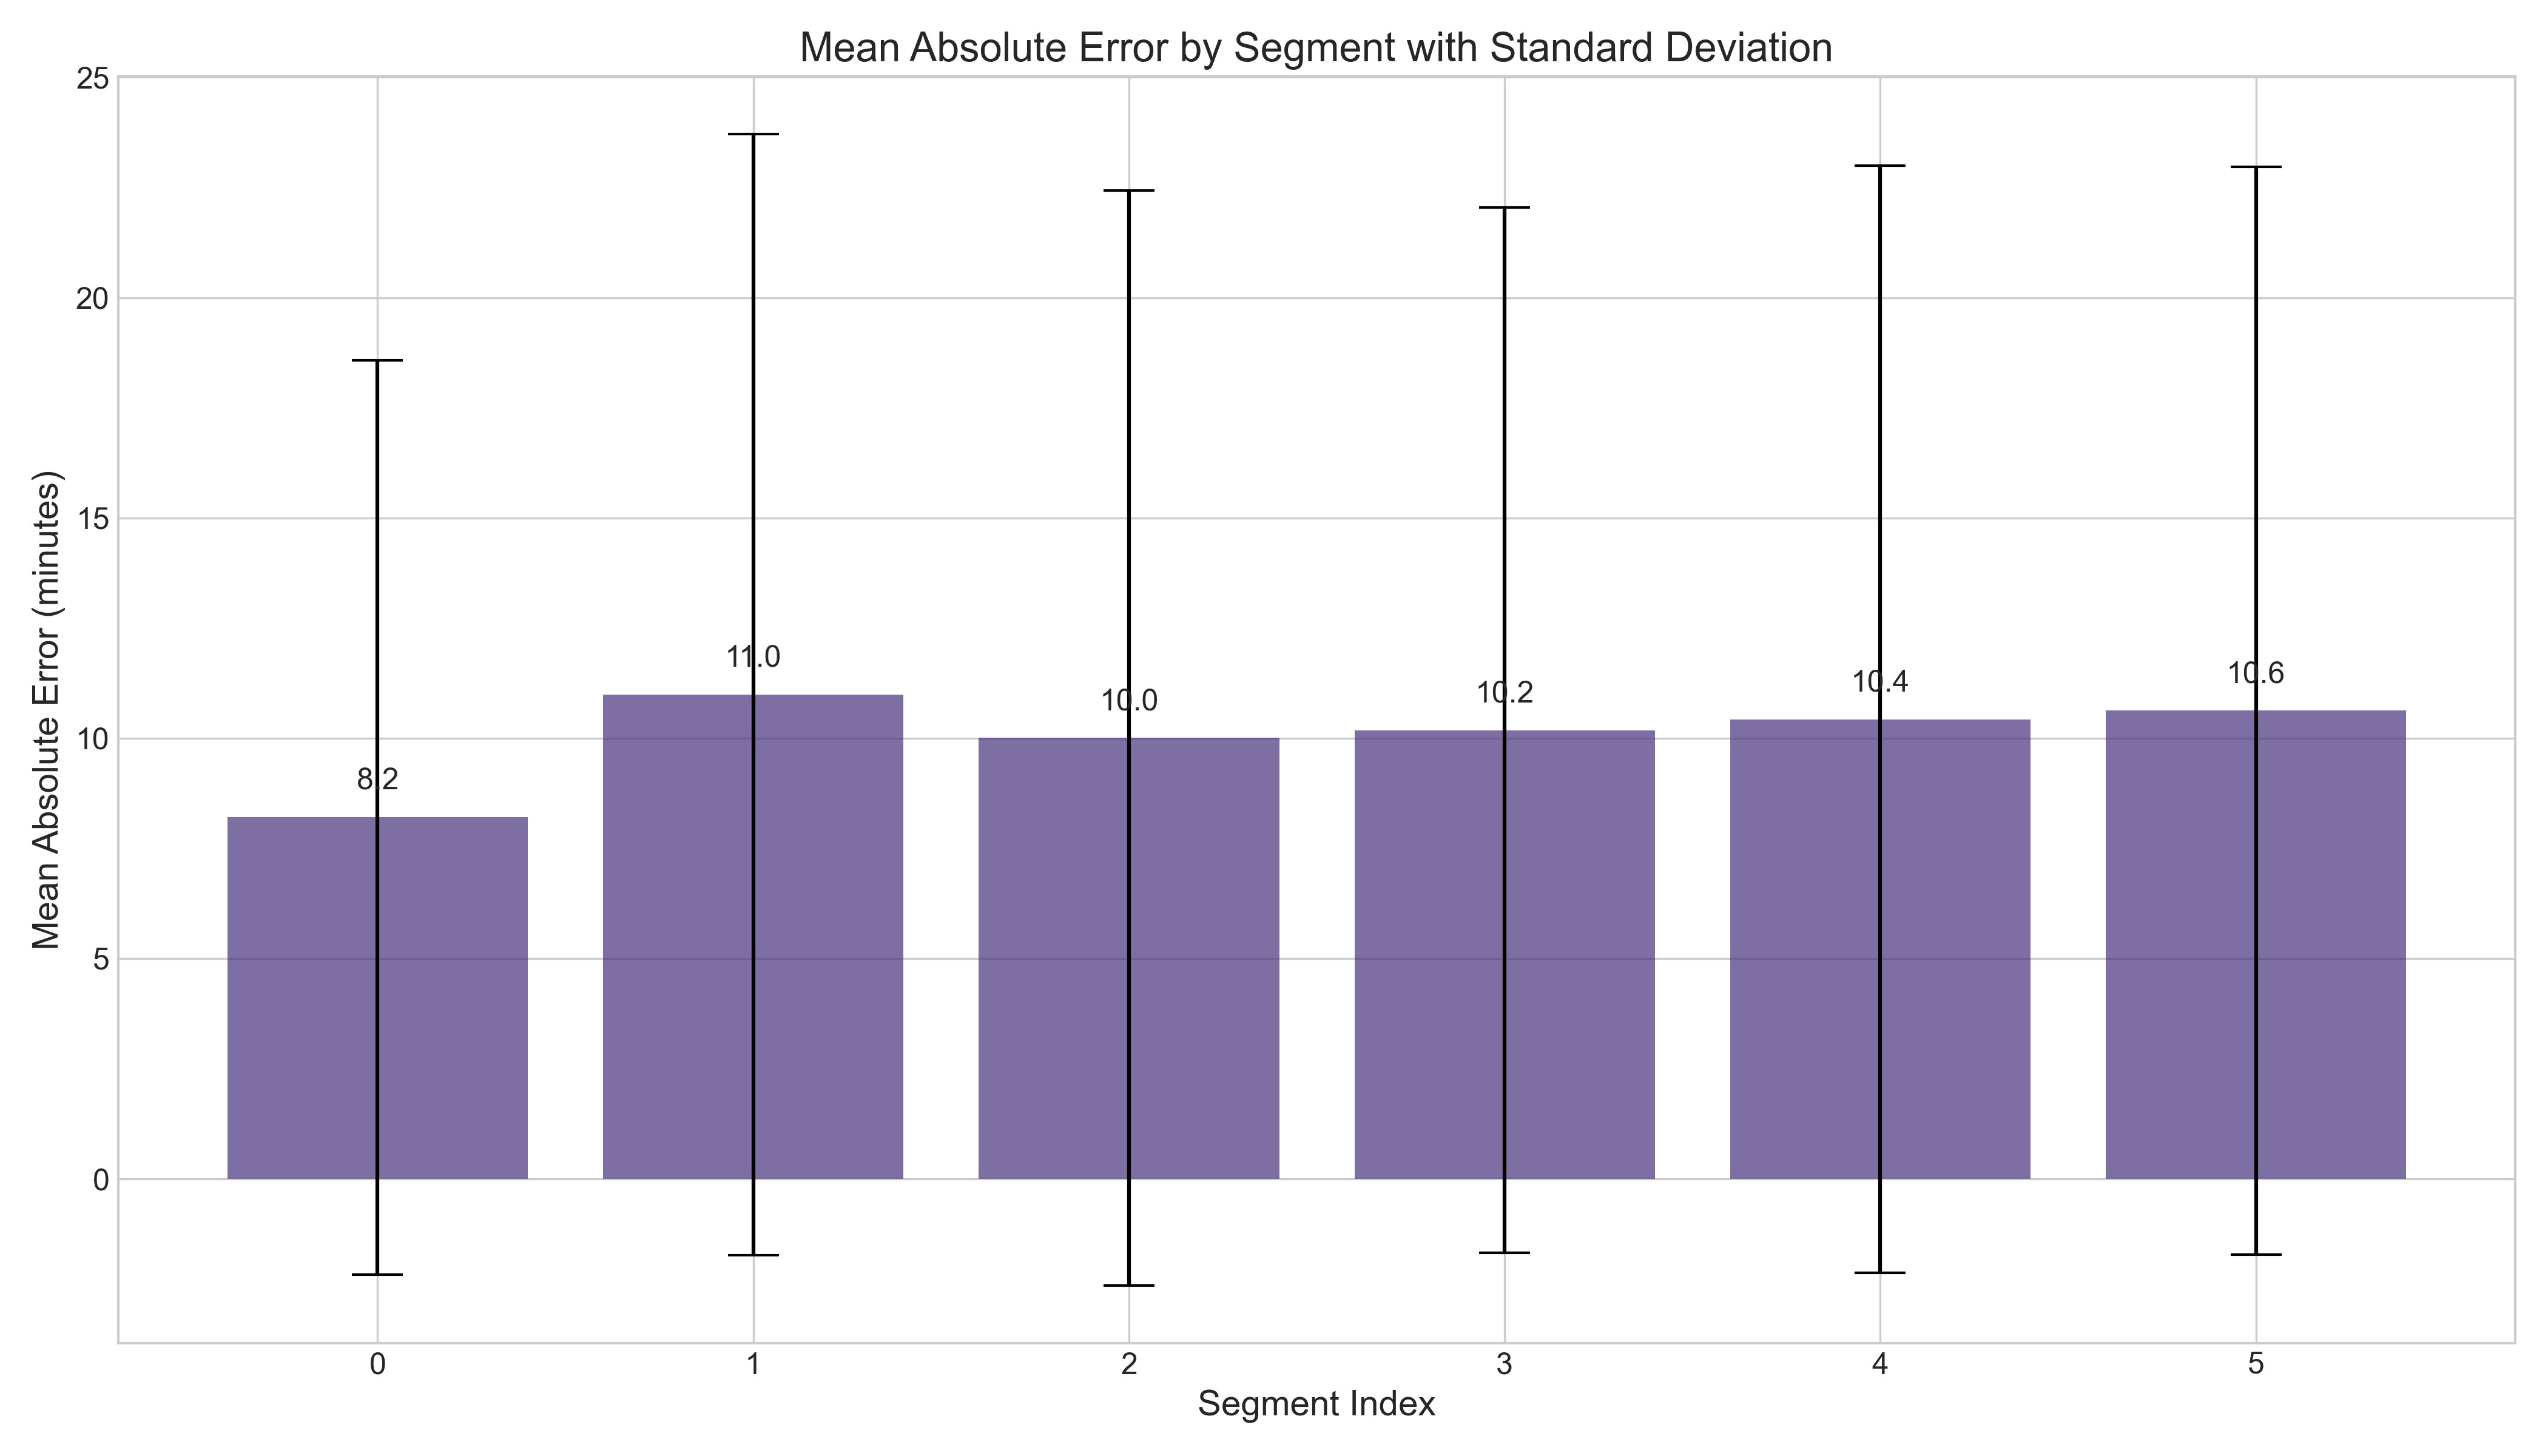
\includegraphics[width=0.7\textwidth]{visualization_results/segment_error_barplot.png}
\caption{Average Error Bar Chart by Segment}
\label{fig:segment_error}
\end{figure}

From the data, it can be seen that the first two segments (Darchen to First Prostration Point, First Prostration Point to Sershong) have smaller prediction errors, while the fourth segment (Second Prostration Point to Dazhen Supply Point) has the largest error despite being the second shortest segment at only 1.5km. This apparent contradiction can be explained by examining the terrain characteristics:

\begin{itemize}
  \item Segments 0 and 1 have low prediction errors (80-100 seconds) and also have straightforward terrain characteristics - segment 0 has a gentle continuous uphill (difficulty level 1) while segment 1 is mainly downhill and flat terrain (difficulty level 0). The predictable nature of these segments makes them easier for the model to accurately estimate.
  
  \item Segment 4, despite its short distance (1.5km), has the highest difficulty rating (5) and shows the largest prediction error (380 seconds). This segment features slight ascent with undulations, which likely introduces variability in pilgrim behavior - some may slow significantly on the undulations while others maintain pace. The high difficulty rating suggests challenging terrain features not fully captured by elevation change alone.
  
  \item Segment 3 has the second-highest error (300 seconds) and is the longest segment (5.5km) with significant elevation gain (+120m) and multiple undulations (difficulty level 4). The combination of length and terrain complexity naturally introduces more variability in completion times.
\end{itemize}

These observations highlight how terrain characteristics beyond simple distance metrics significantly impact prediction accuracy.

\subsection{Comparison of Predicted vs. Actual Values}

Figure \ref{fig:pred_vs_actual} shows a scatter plot comparing predicted times with actual times. The points are distributed around the ideal line (y=x), indicating that the predictions are generally accurate. However, as time increases, the degree of dispersion in predictions also increases, indicating that for longer time predictions, model accuracy decreases slightly.

\begin{figure}[H]
\centering
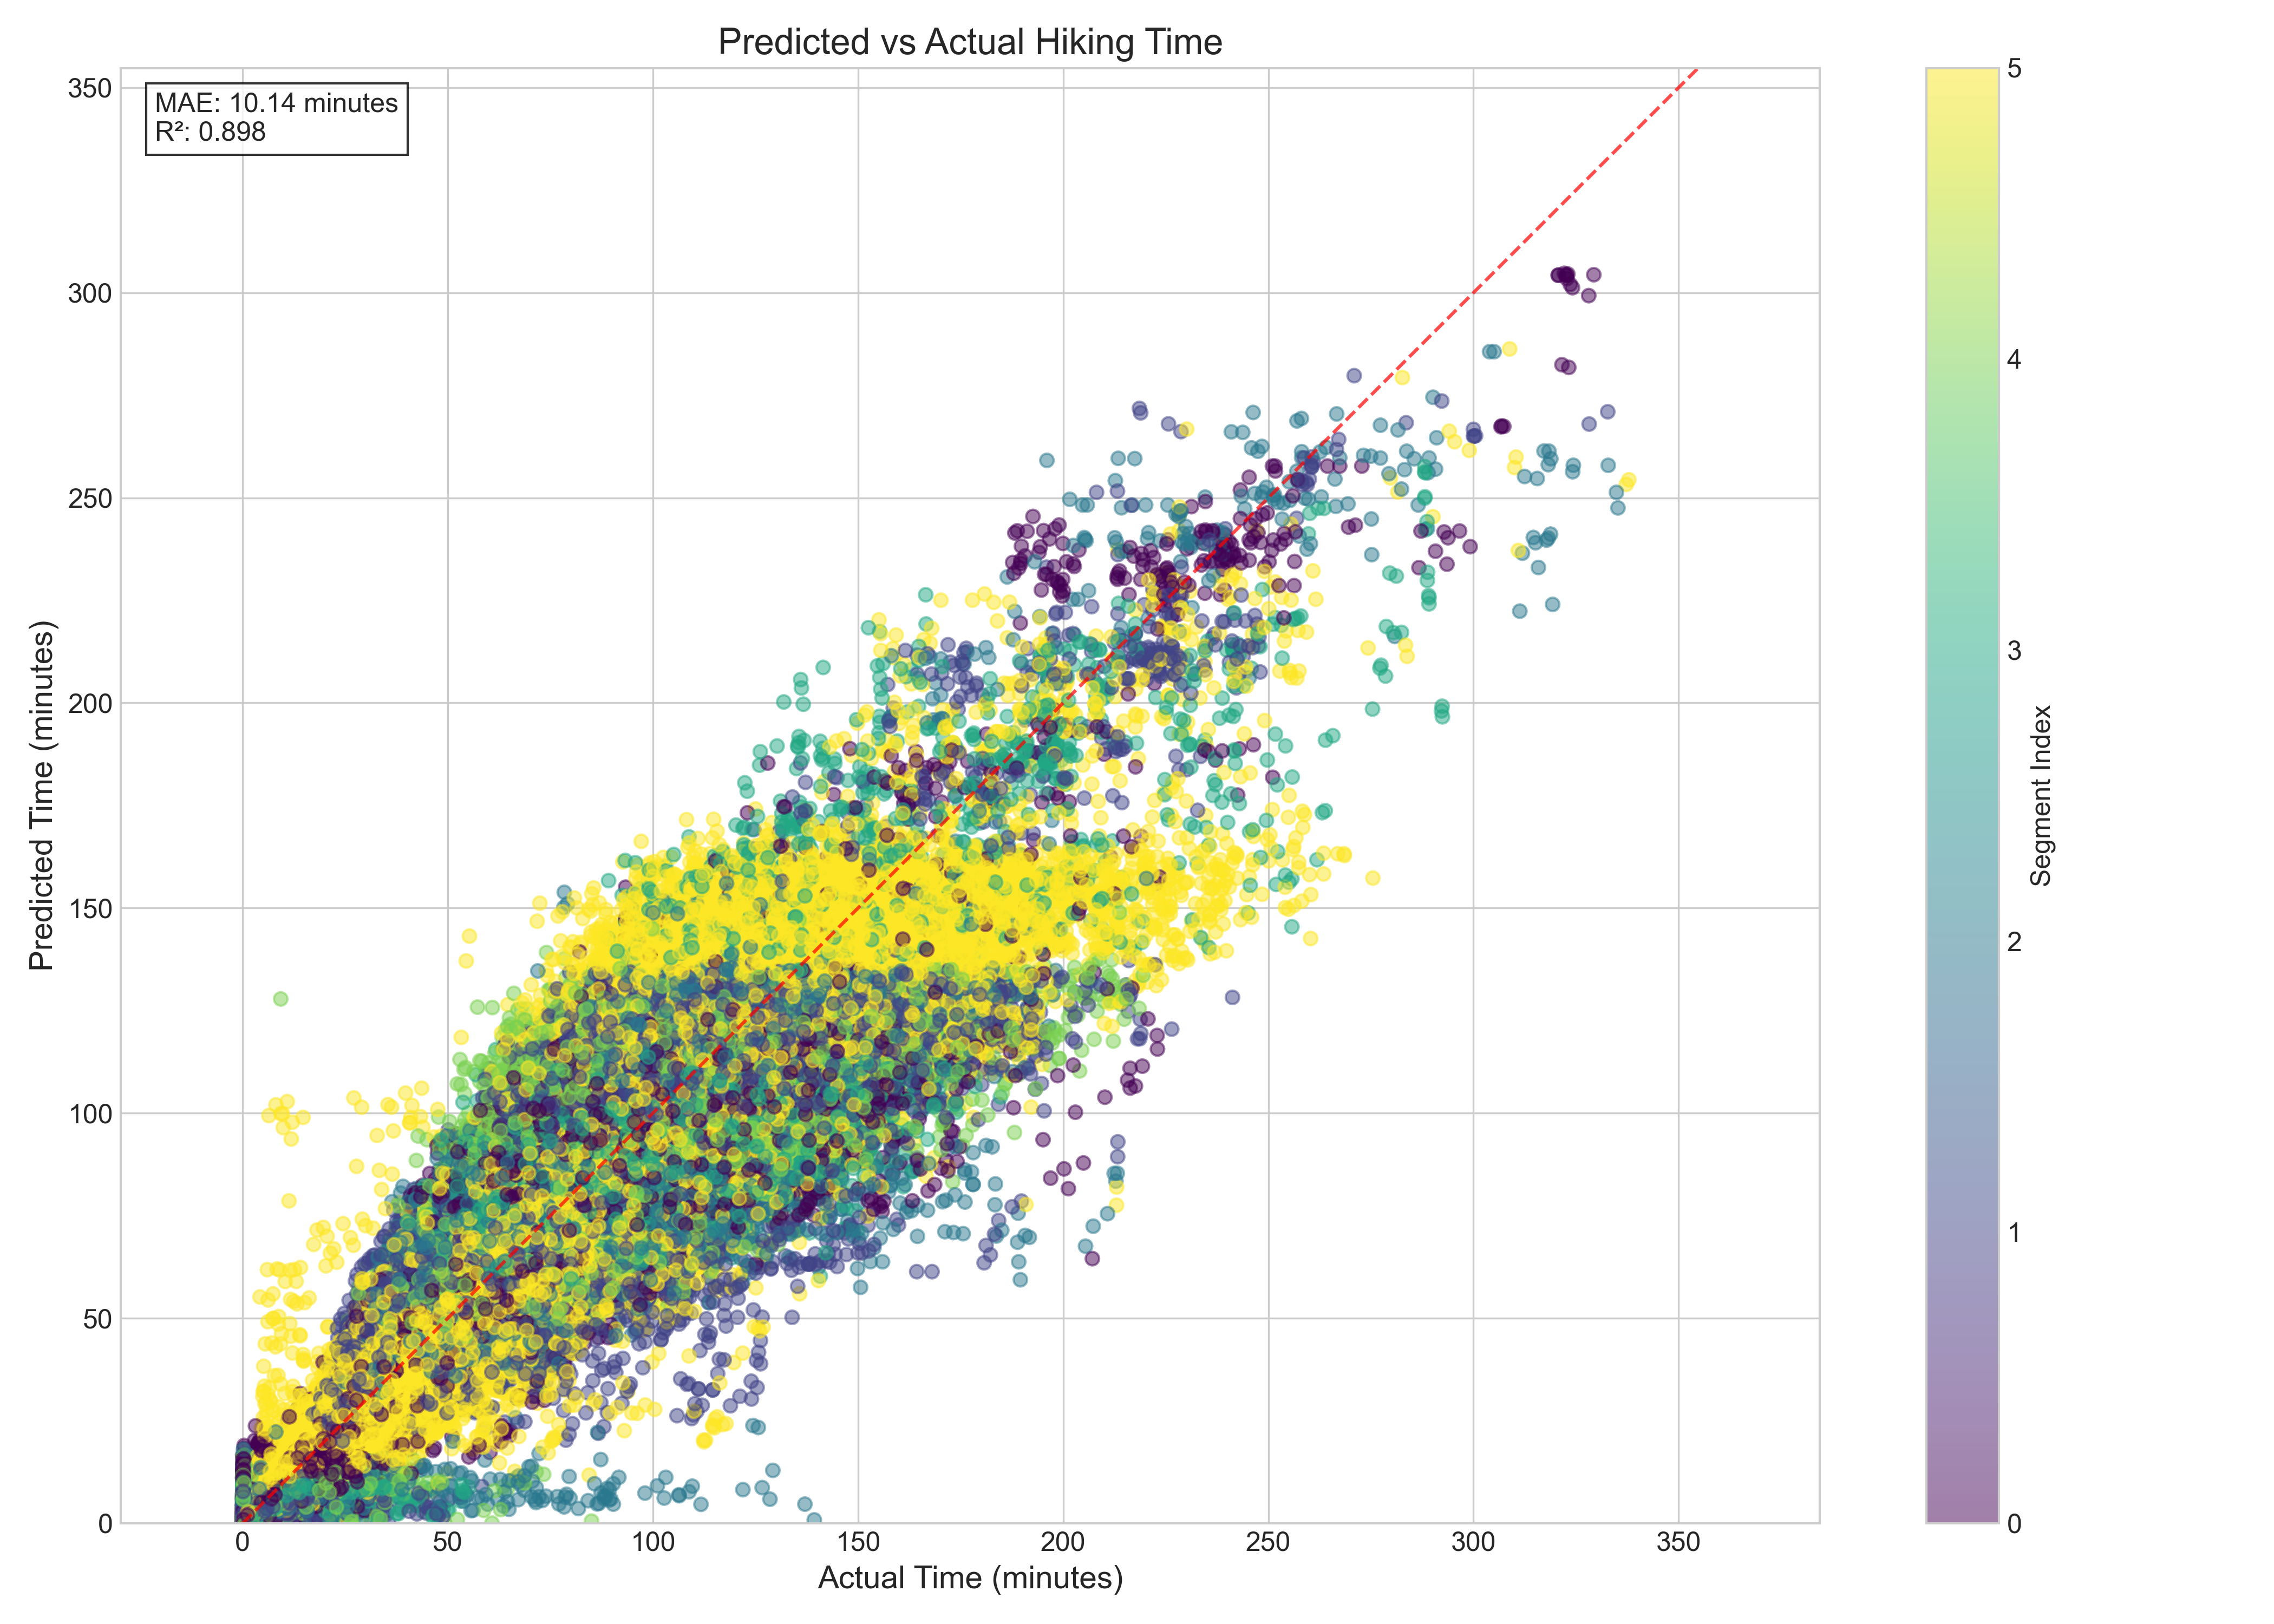
\includegraphics[width=0.65\textwidth]{visualization_results/prediction_vs_actual.png}
\caption{Scatter Plot of Predicted vs. Actual Values}
\label{fig:pred_vs_actual}
\end{figure}

Figure \ref{fig:pred_by_dest} further shows prediction performance grouped by destination. It can be seen that the model performs differently for different destinations, but overall maintains high accuracy.

\begin{figure}[H]
\centering
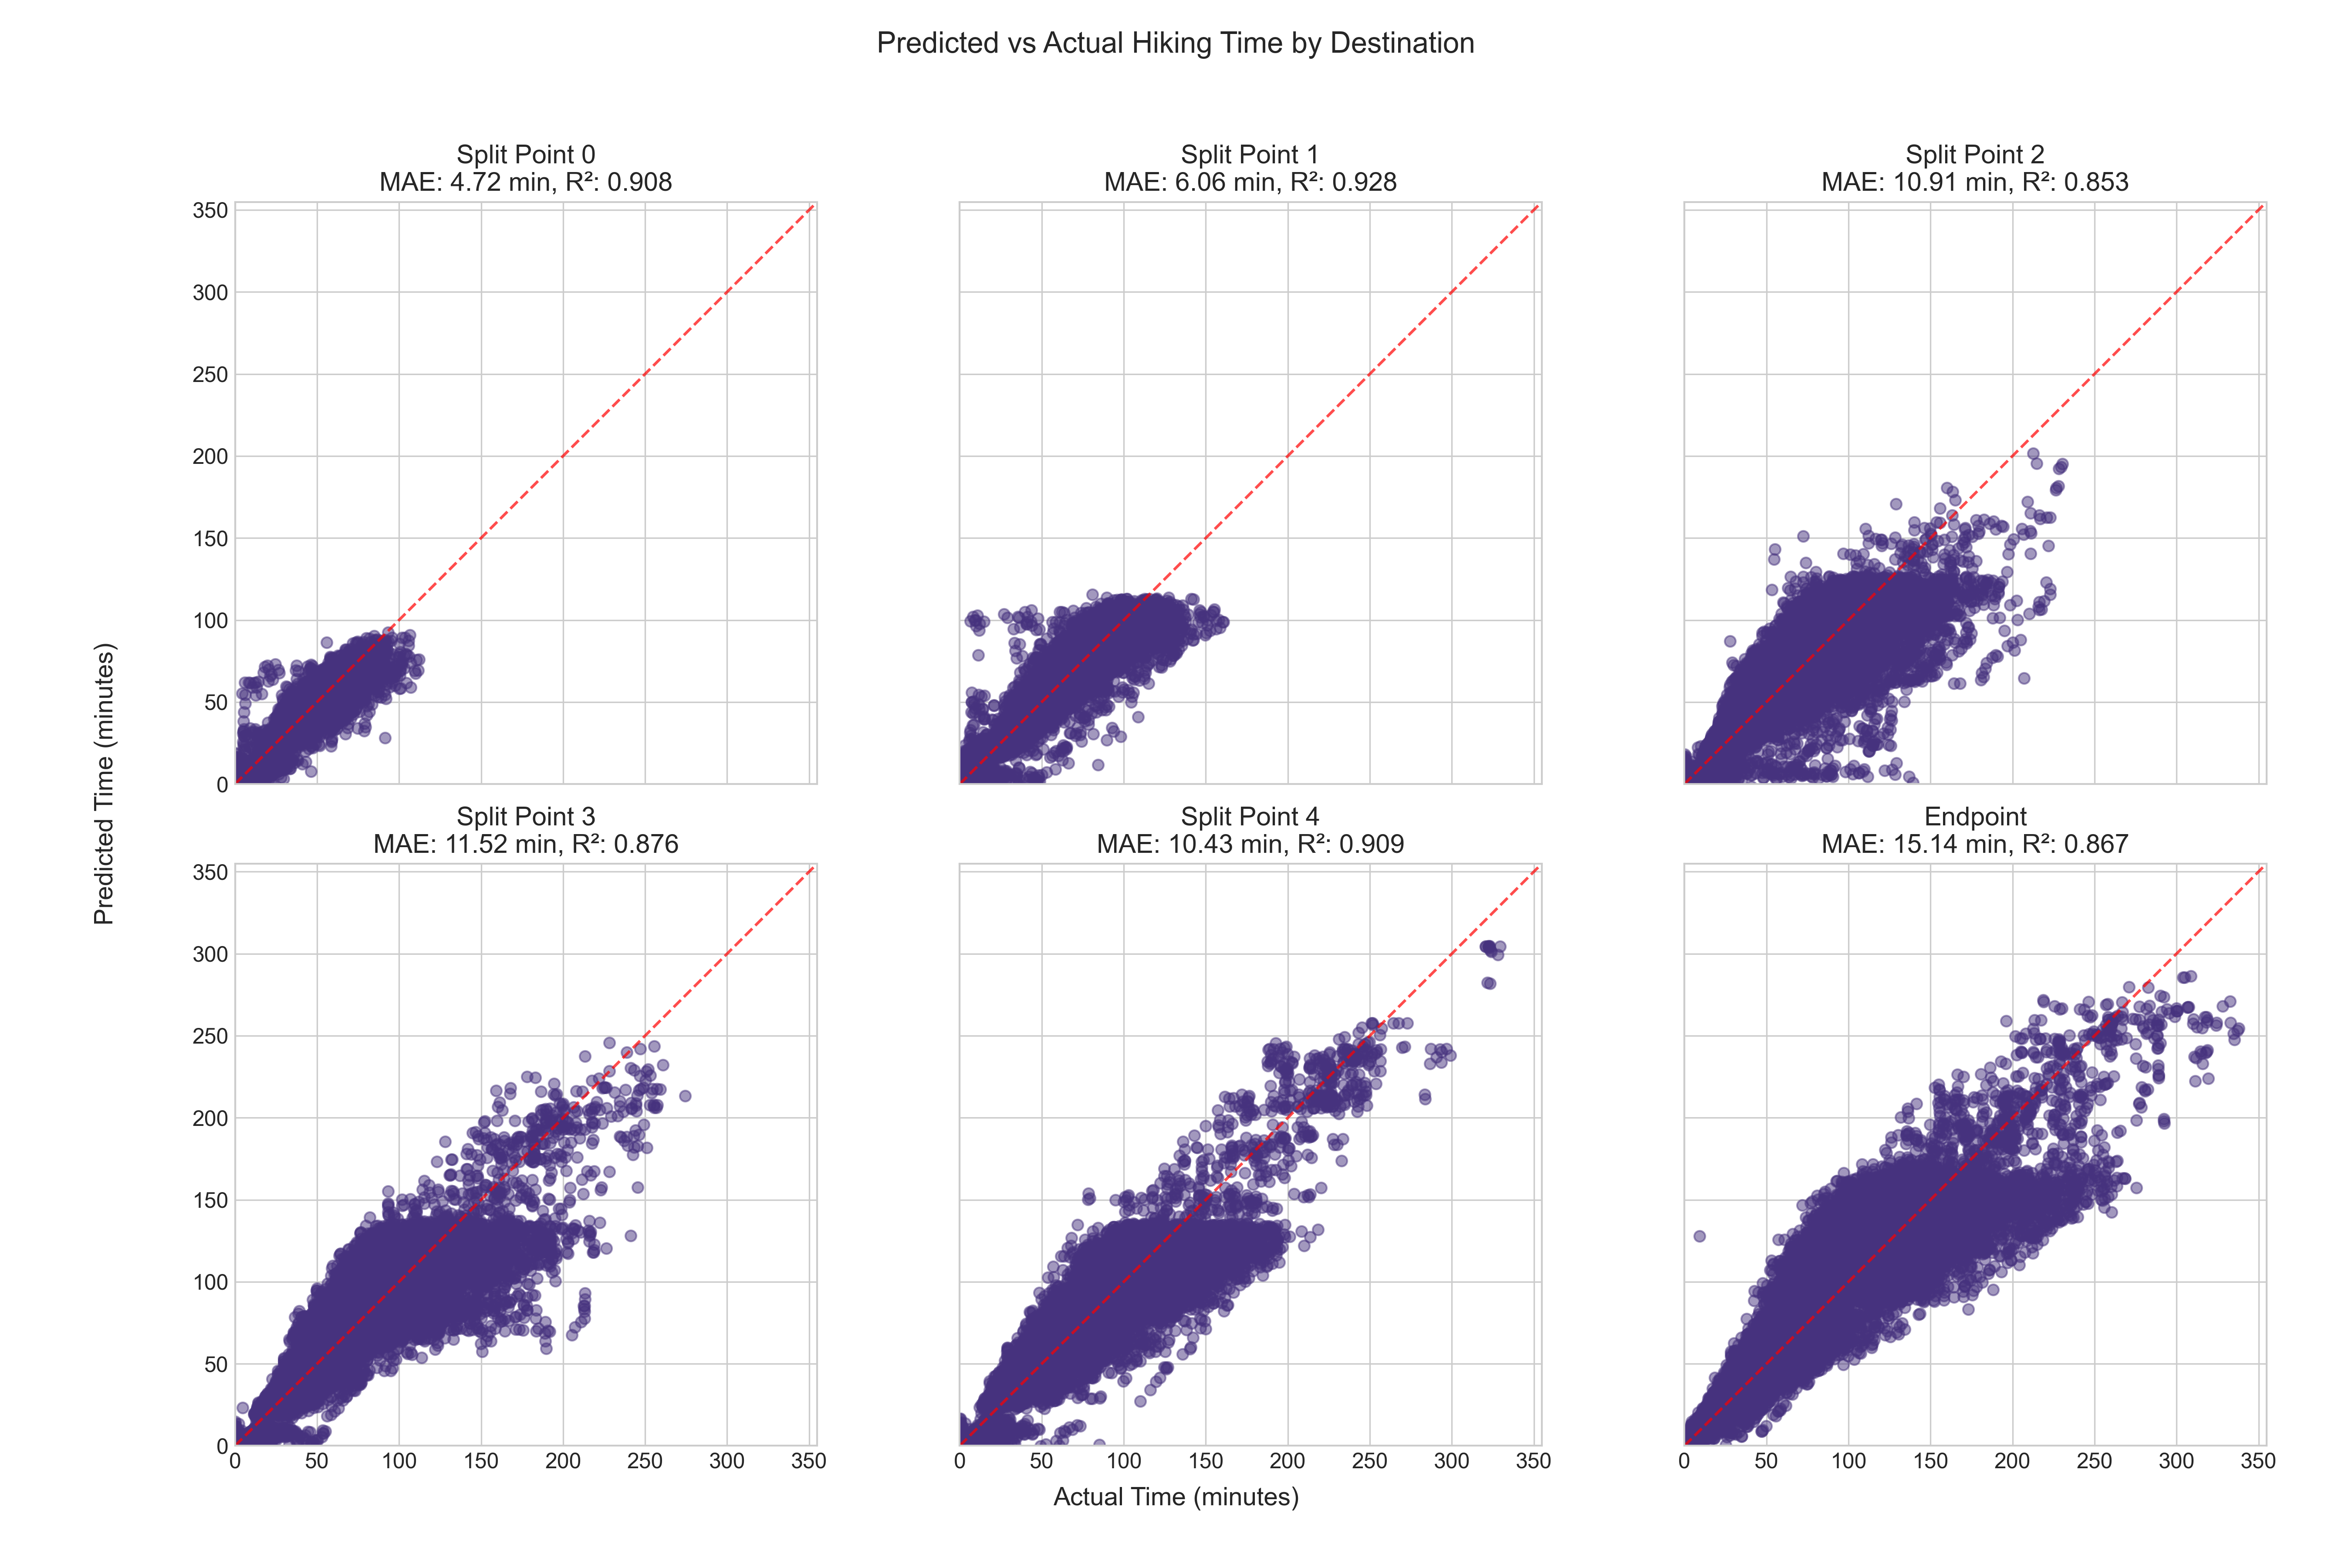
\includegraphics[width=0.8\textwidth]{visualization_results/prediction_vs_actual_by_destination.png}
\caption{Predicted vs. Actual Values Grouped by Destination}
\label{fig:pred_by_dest}
\end{figure}

\section{Feature Importance Analysis}

\subsection{Key Prediction Factors}

Based on XGBoost's feature importance evaluation (Gain metric), we identified the features with the most influence on prediction, as shown in Table \ref{tab:feature_importance} and Figure \ref{fig:feature_importance}:

\begin{table}[H]
\centering
\caption{Feature Importance Ranking}
\label{tab:feature_importance}
\begin{tabular}{lr}
\toprule
Feature & Gain Ratio (\%) \\
\midrule
dist\_to\_dest & 35.55 \\
dest\_5 & 19.21 \\
segment\_4 & 10.32 \\
destination\_idx & 5.48 \\
difficulty\_level & 4.63 \\
gradient & 2.13 \\
speed & 1.87 \\
time\_of\_day & 1.24 \\
season & 0.95 \\
\bottomrule
\end{tabular}
\end{table}

\begin{figure}[H]
\centering
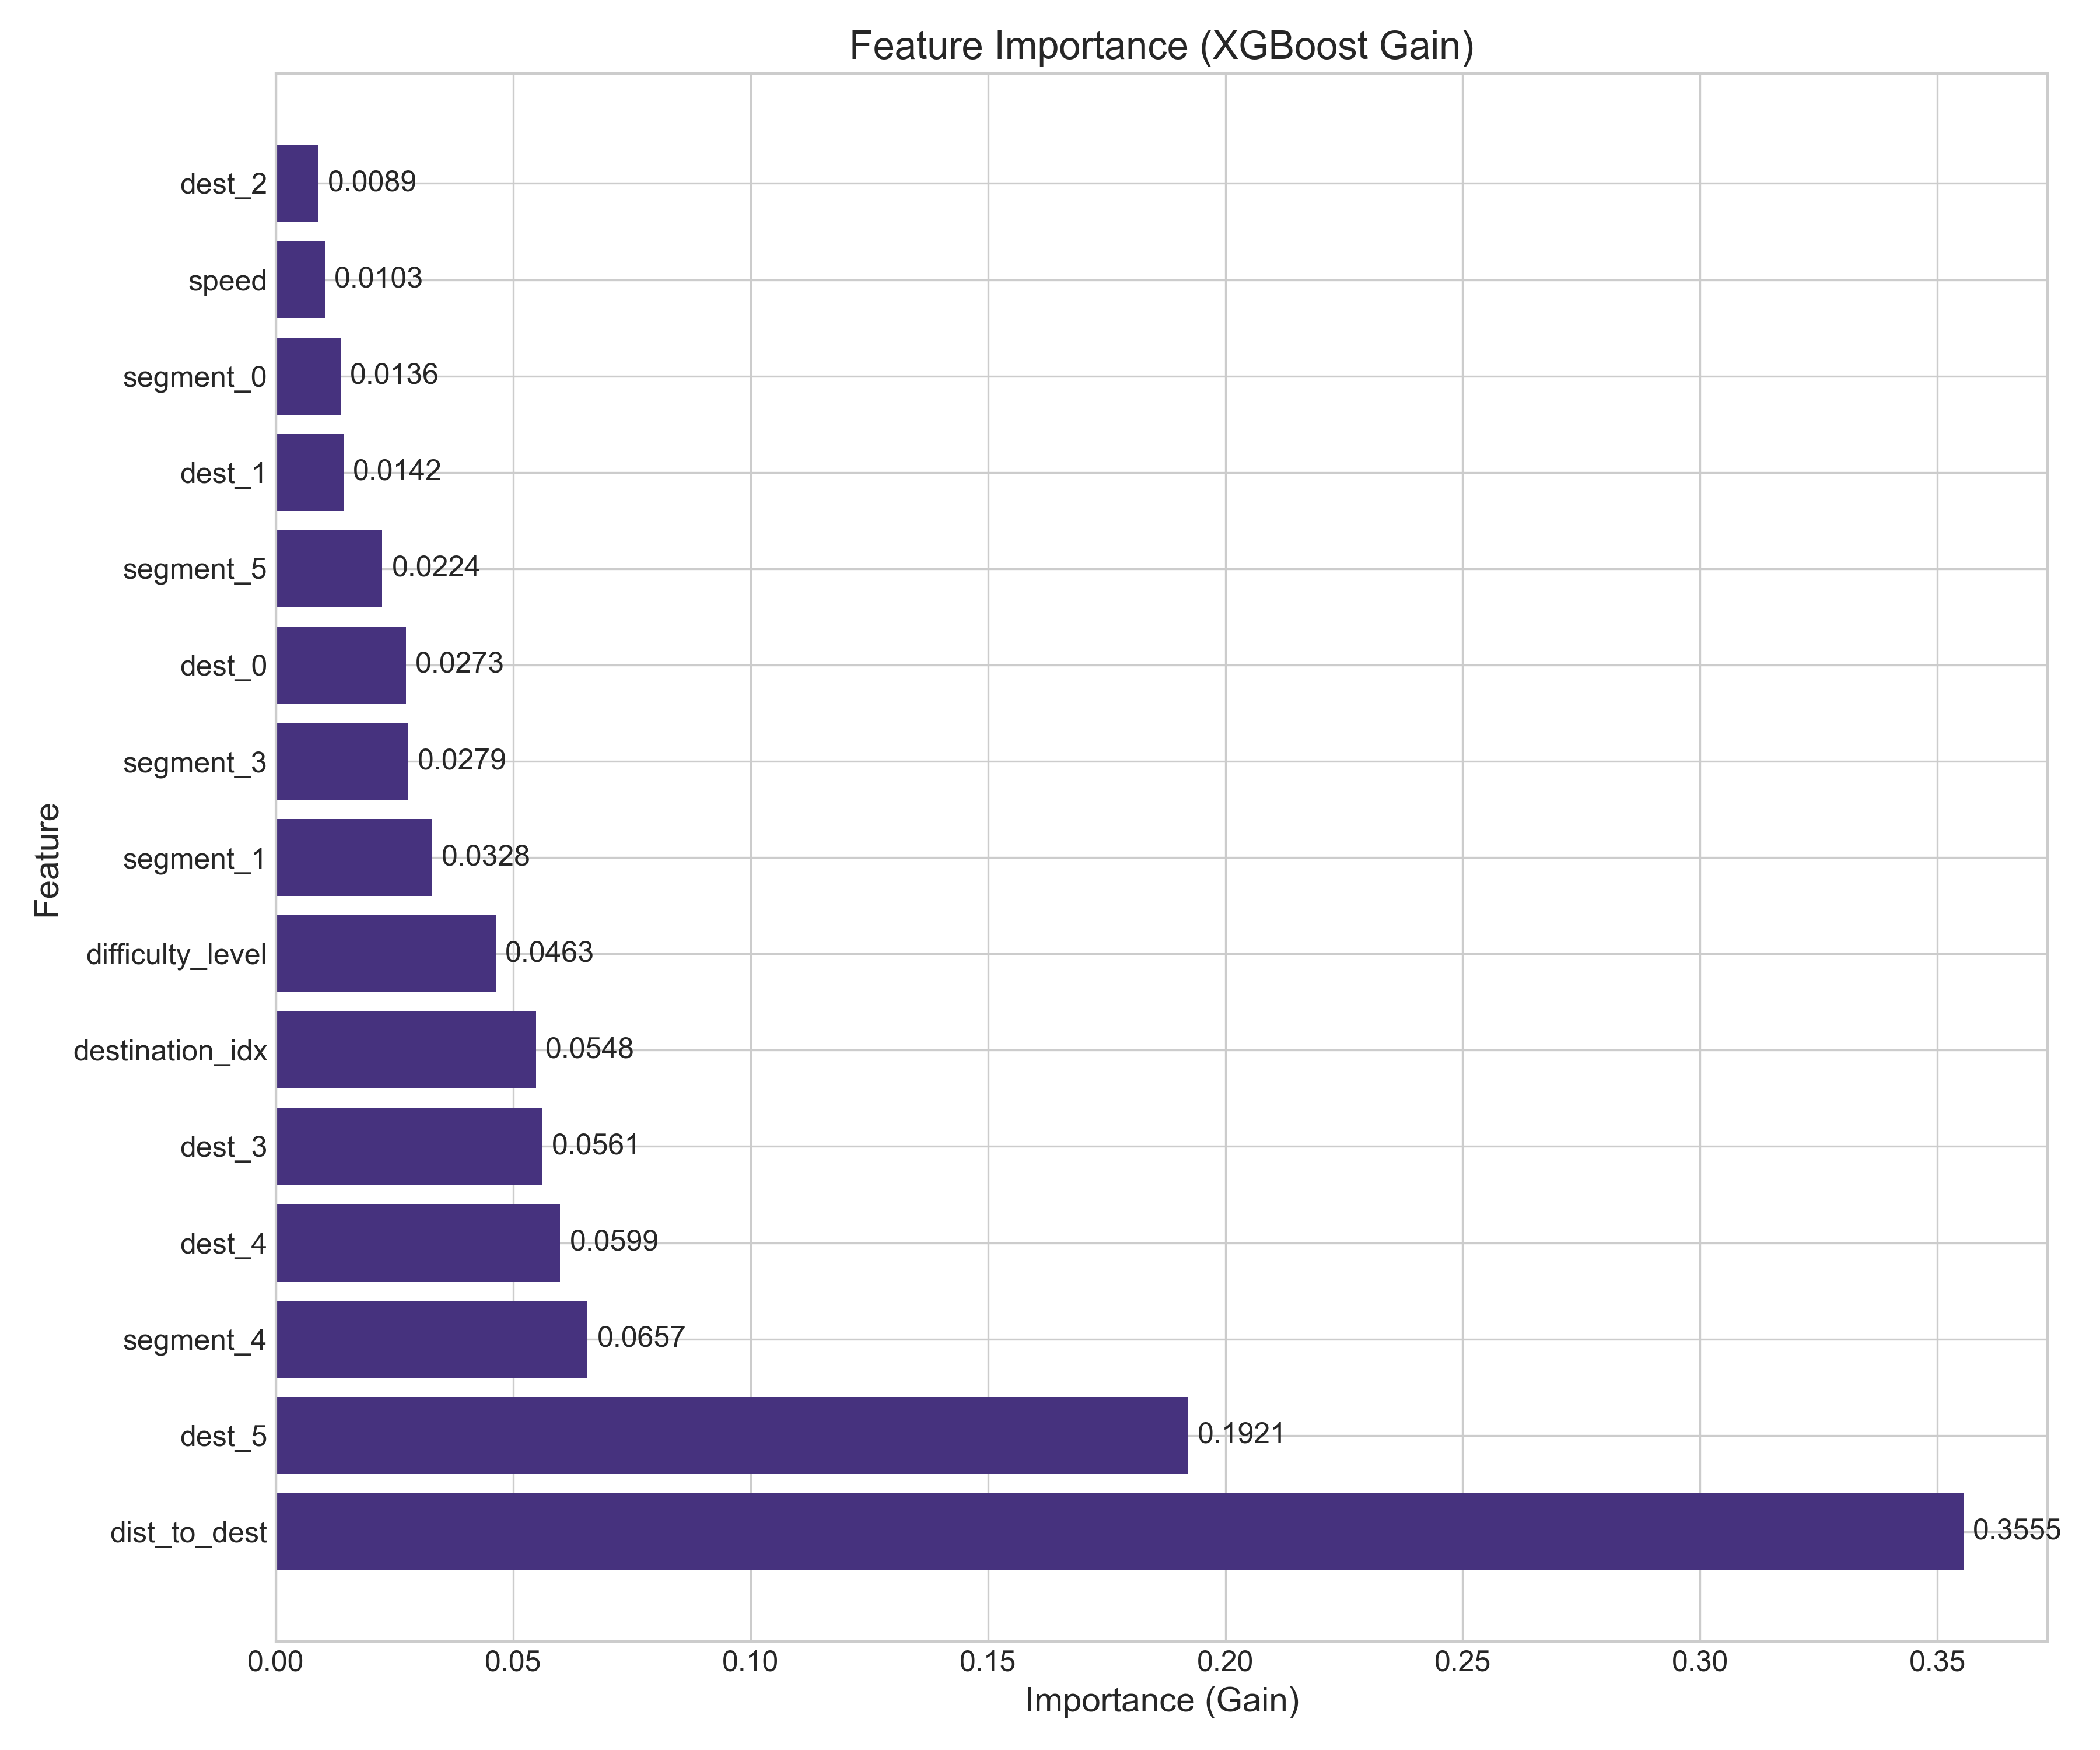
\includegraphics[width=0.8\textwidth]{visualization_results/feature_importance.png}
\caption{Feature Importance Bar Chart}
\label{fig:feature_importance}
\end{figure}

From the results, we can see:

\begin{itemize}
  \item \textbf{Distance Factor}: Distance to destination (dist\_to\_dest) is the most important prediction factor, contributing over 35\% of the predictive power. This aligns with our terrain analysis, as the total route spans approximately 19.8km with varying elevation profiles.
  
  \item \textbf{Destination Features}: Specific destinations (dest\_5, i.e., the final segment to Gangjia/Zhire Temple) have significant influence (19.21\%), which correlates with its challenging terrain characteristics - a 4.3-4.7km stretch with substantial elevation gain (+190/+160m). This segment requires pilgrims to navigate a gradual but persistent ascent, creating unique time requirements compared to other segments.
  
  \item \textbf{Segment Features}: segment\_4 (Second Prostration Point to Dazhen Supply Point) contributes 10.32\% to prediction power despite being only 1.5km long. This disproportionate importance is explained by its highest difficulty rating (5) and its undulating terrain. The model correctly identifies that this short segment introduces significant variability in hiking times.
  
  \item \textbf{Environmental Factors}: Difficulty level (4.63\%) and gradient (2.13\%) together contribute about 7\% of the predictive power. This reflects how the varying terrain across segments - from flat paths (segment 2) to multiple undulations (segments 3 and 4) - significantly impacts travel times beyond what distance alone would predict.
  
  \item \textbf{Time Factors}: Time of day (1.24\%) and season (0.95\%), although relatively low in importance, still contribute to prediction. This suggests environmental conditions like temperature, daylight, and seasonal weather patterns affect pilgrim pace, particularly in the more challenging segments with higher elevation changes.
\end{itemize}

The model's feature importance aligns remarkably well with the physical characteristics of the route segments, demonstrating that the algorithm has successfully captured the real-world factors that influence hiking times.

\subsection{SHAP Analysis for Model Interpretability}

To gain deeper insights into how our model makes predictions, we employed SHAP (SHapley Additive exPlanations) analysis. SHAP values, based on cooperative game theory, provide a unified measure of feature importance that is consistent, locally accurate, and has solid theoretical foundations.

\begin{figure}[H]
\centering
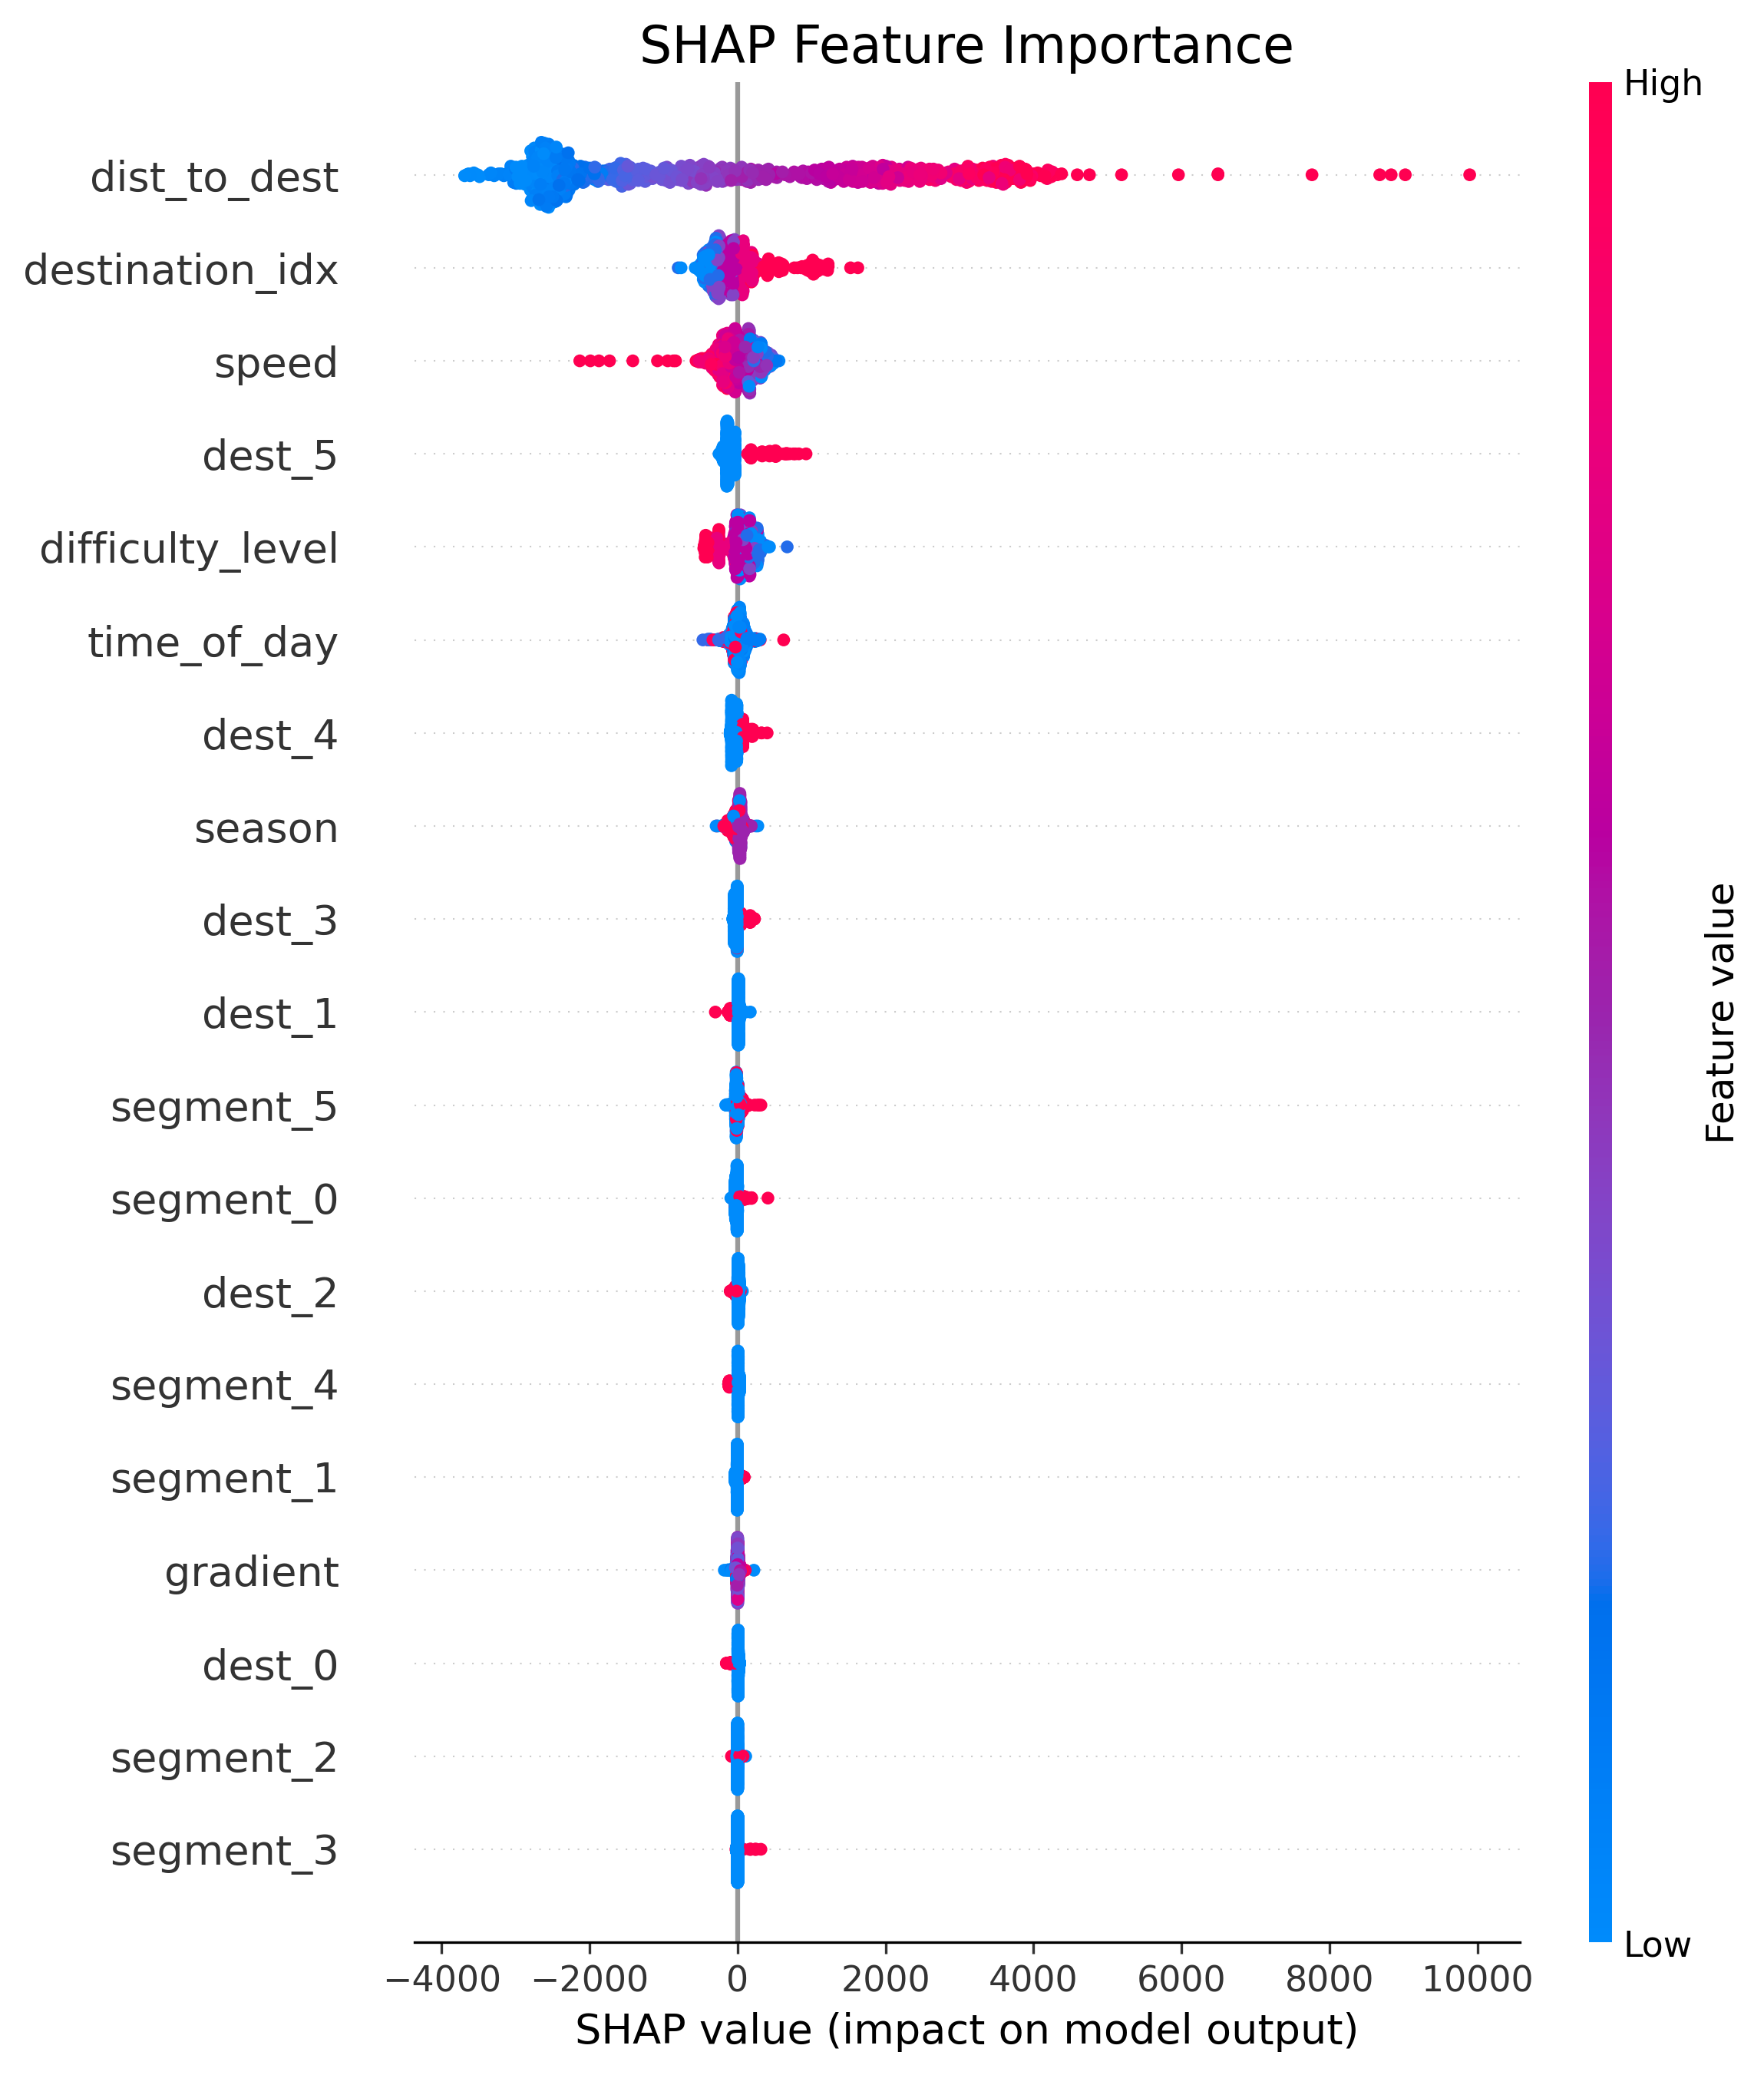
\includegraphics[width=0.9\textwidth]{visualization_results/shap_summary_plot.png}
\caption{SHAP Summary Plot Showing Feature Impact on Predictions}
\label{fig:shap_summary}
\end{figure}

Figure \ref{fig:shap_summary} shows the SHAP summary plot, which reveals not only the magnitude of each feature's impact (horizontal axis) but also the direction of impact (color). Red points indicate higher feature values, while blue points indicate lower values. Several key insights emerge:

\begin{itemize}
  \item \textbf{Distance Effect Direction}: Lower distances to destination (blue points) consistently push predictions downward (shorter times), while greater distances (red points) push predictions upward (longer times), confirming the intuitive relationship between distance and hiking time.
  
  \item \textbf{Segment-Specific Effects}: The segment\_4 feature shows a strong positive impact when present (red points clustered on the right), confirming our earlier finding that this challenging segment disproportionately increases hiking time despite its short length.
  
  \item \textbf{Destination Variability}: The dest\_5 feature shows both positive and negative impacts, indicating that this destination's effect on prediction is context-dependent and interacts with other features.
  
  \item \textbf{Gradient Impact Pattern}: The gradient feature shows a clear pattern where steeper gradients (red) increase predicted time while downhill sections (blue) decrease it, with a wider spread of effects than might be suggested by its global importance rank.
\end{itemize}

\begin{figure}[H]
\centering
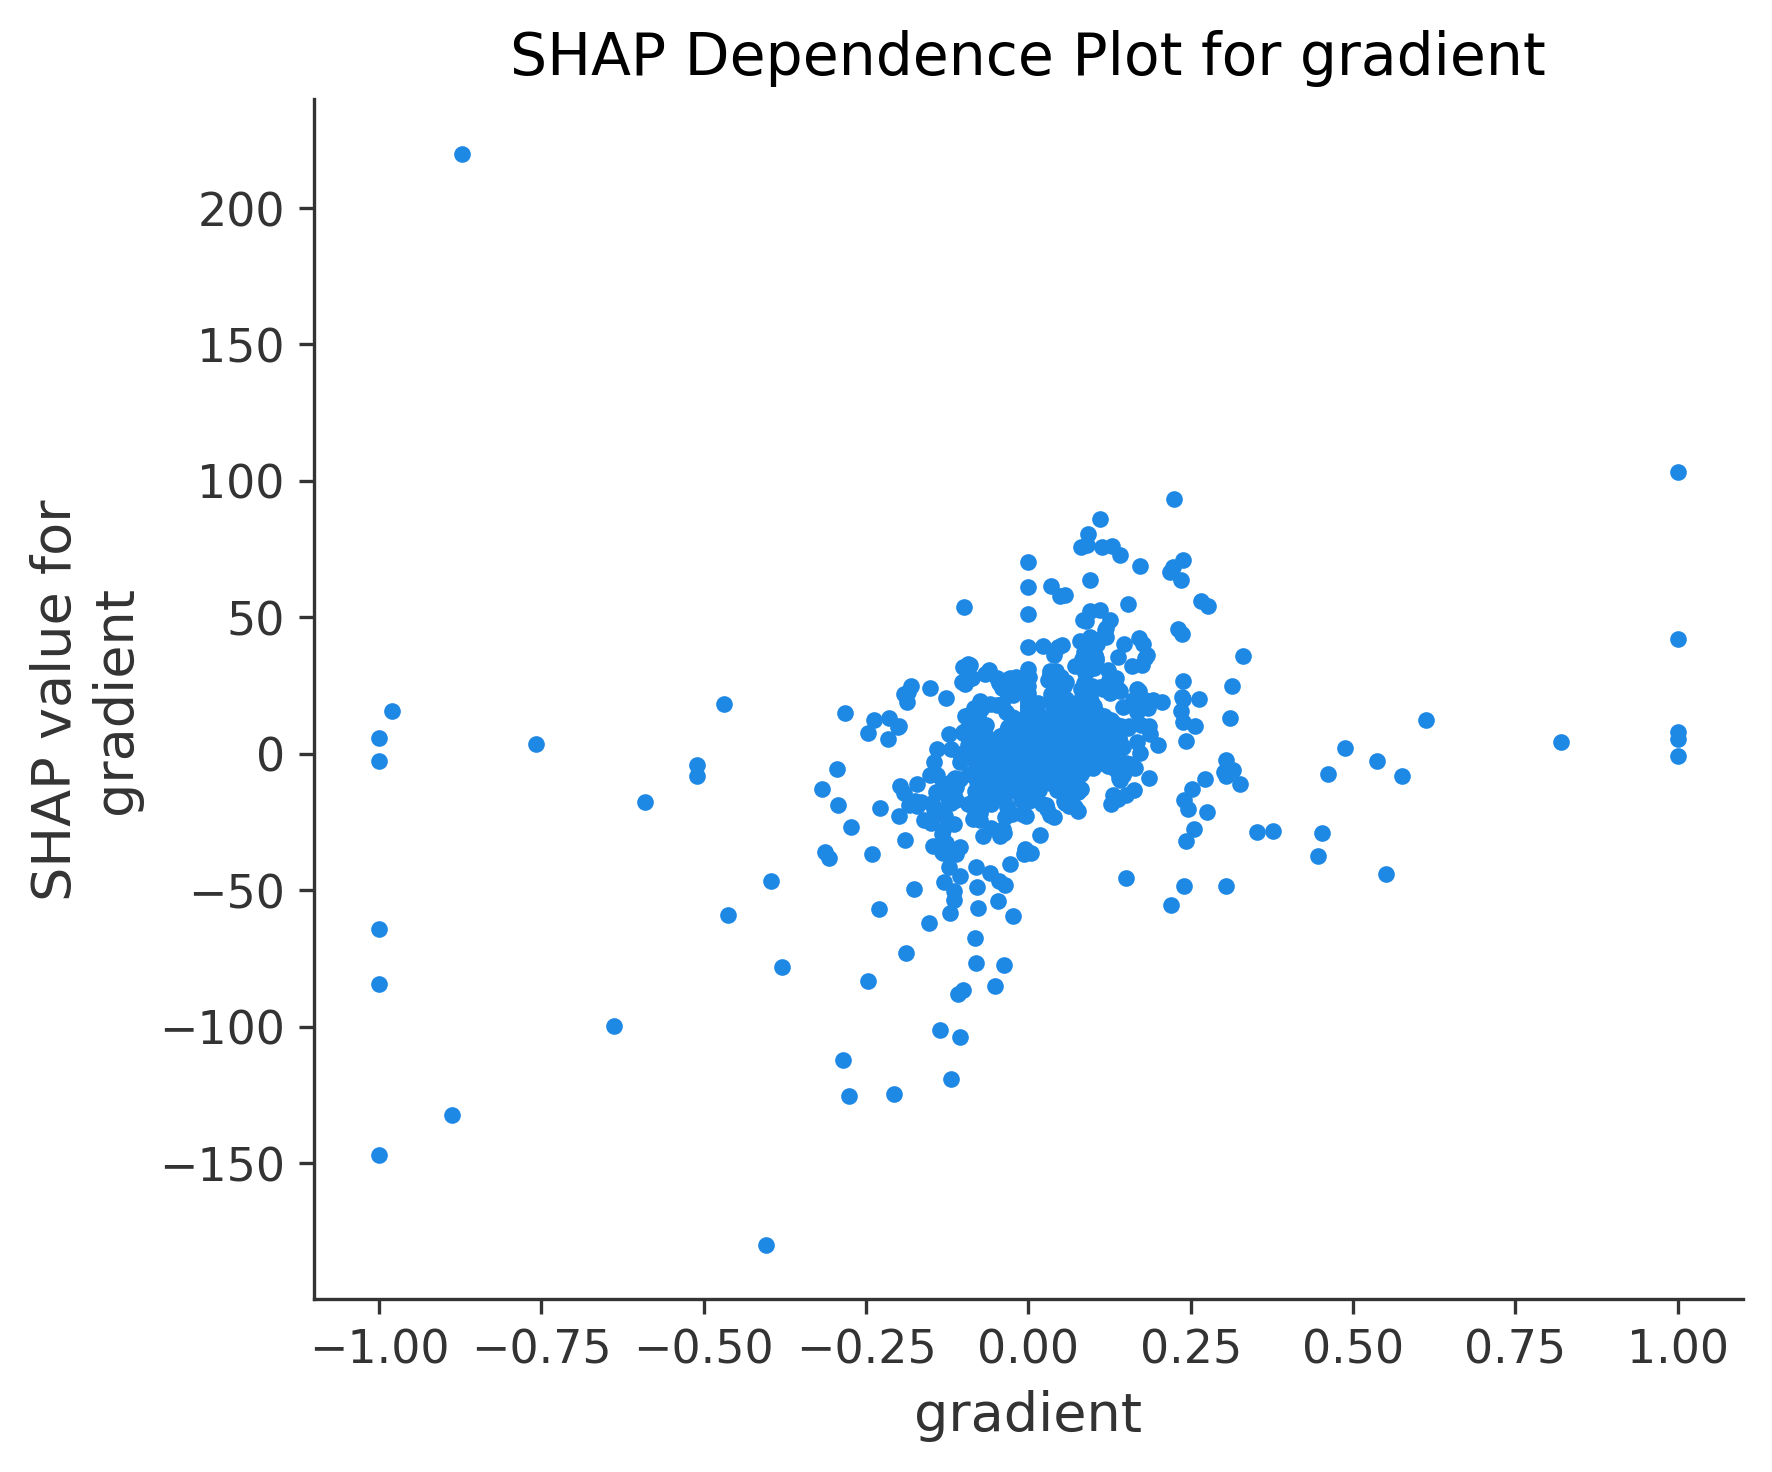
\includegraphics[width=0.8\textwidth]{visualization_results/shap_dependence_gradient.png}
\caption{SHAP Dependence Plot for Gradient Feature}
\label{fig:shap_gradient}
\end{figure}

The dependence plot in Figure \ref{fig:shap_gradient} further illustrates how the gradient feature affects predictions. The non-linear relationship shows that moderate uphill gradients have a relatively small impact, but as the gradient increases beyond certain thresholds, its effect on hiking time increases dramatically. This explains why segment 4, despite having only a +30m elevation change, has such high difficulty and prediction error - the localized steep sections within this segment have an outsized impact on hiking time.

\begin{figure}[H]
\centering
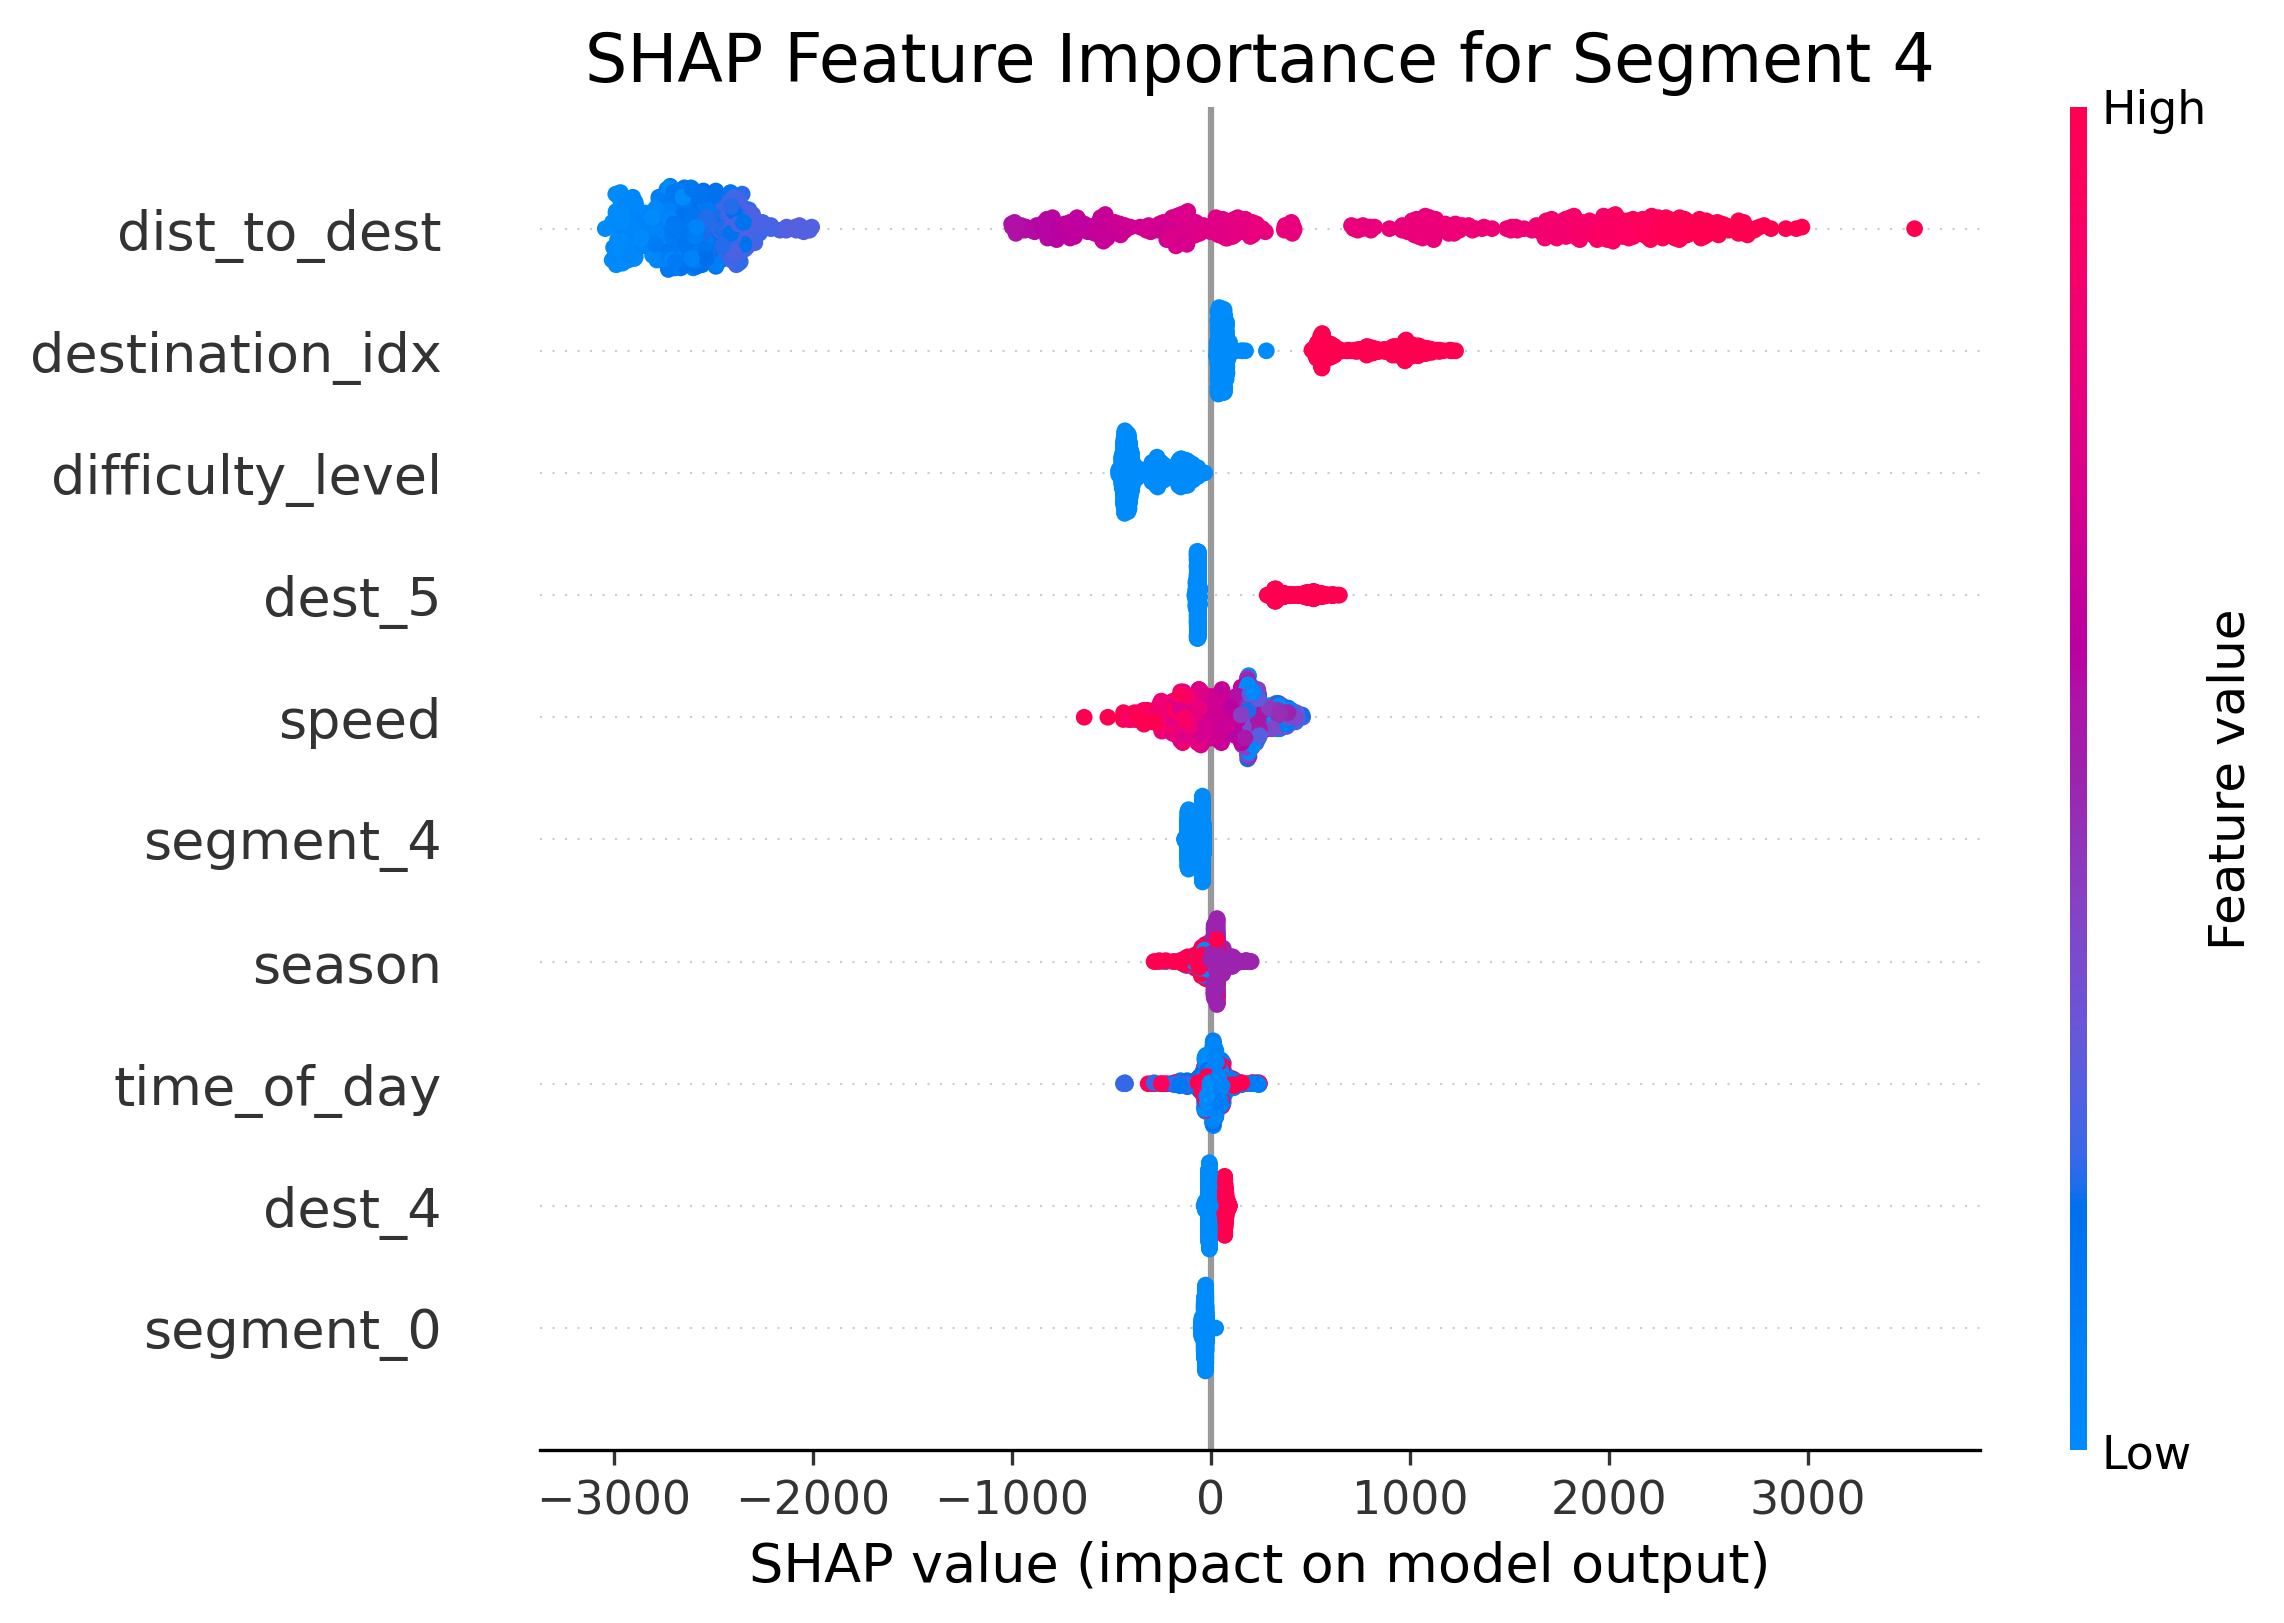
\includegraphics[width=0.8\textwidth]{visualization_results/segment_shap/shap_summary_segment_4.png}
\caption{SHAP Feature Importance for Segment 4 (Second Prostration Point to Dazhen Supply Point)}
\label{fig:shap_segment4}
\end{figure}

Figure \ref{fig:shap_segment4} shows the SHAP analysis specific to segment 4, which has the highest difficulty rating. Interestingly, within this segment, the difficulty\_level feature becomes more prominent compared to the global model, and the gradient feature shows a wider range of impacts. This segment-specific analysis reveals that the terrain characteristics have different relative importances within each segment, explaining why a one-size-fits-all prediction approach would be less effective than our segment-aware model.

\begin{figure}[H]
\centering
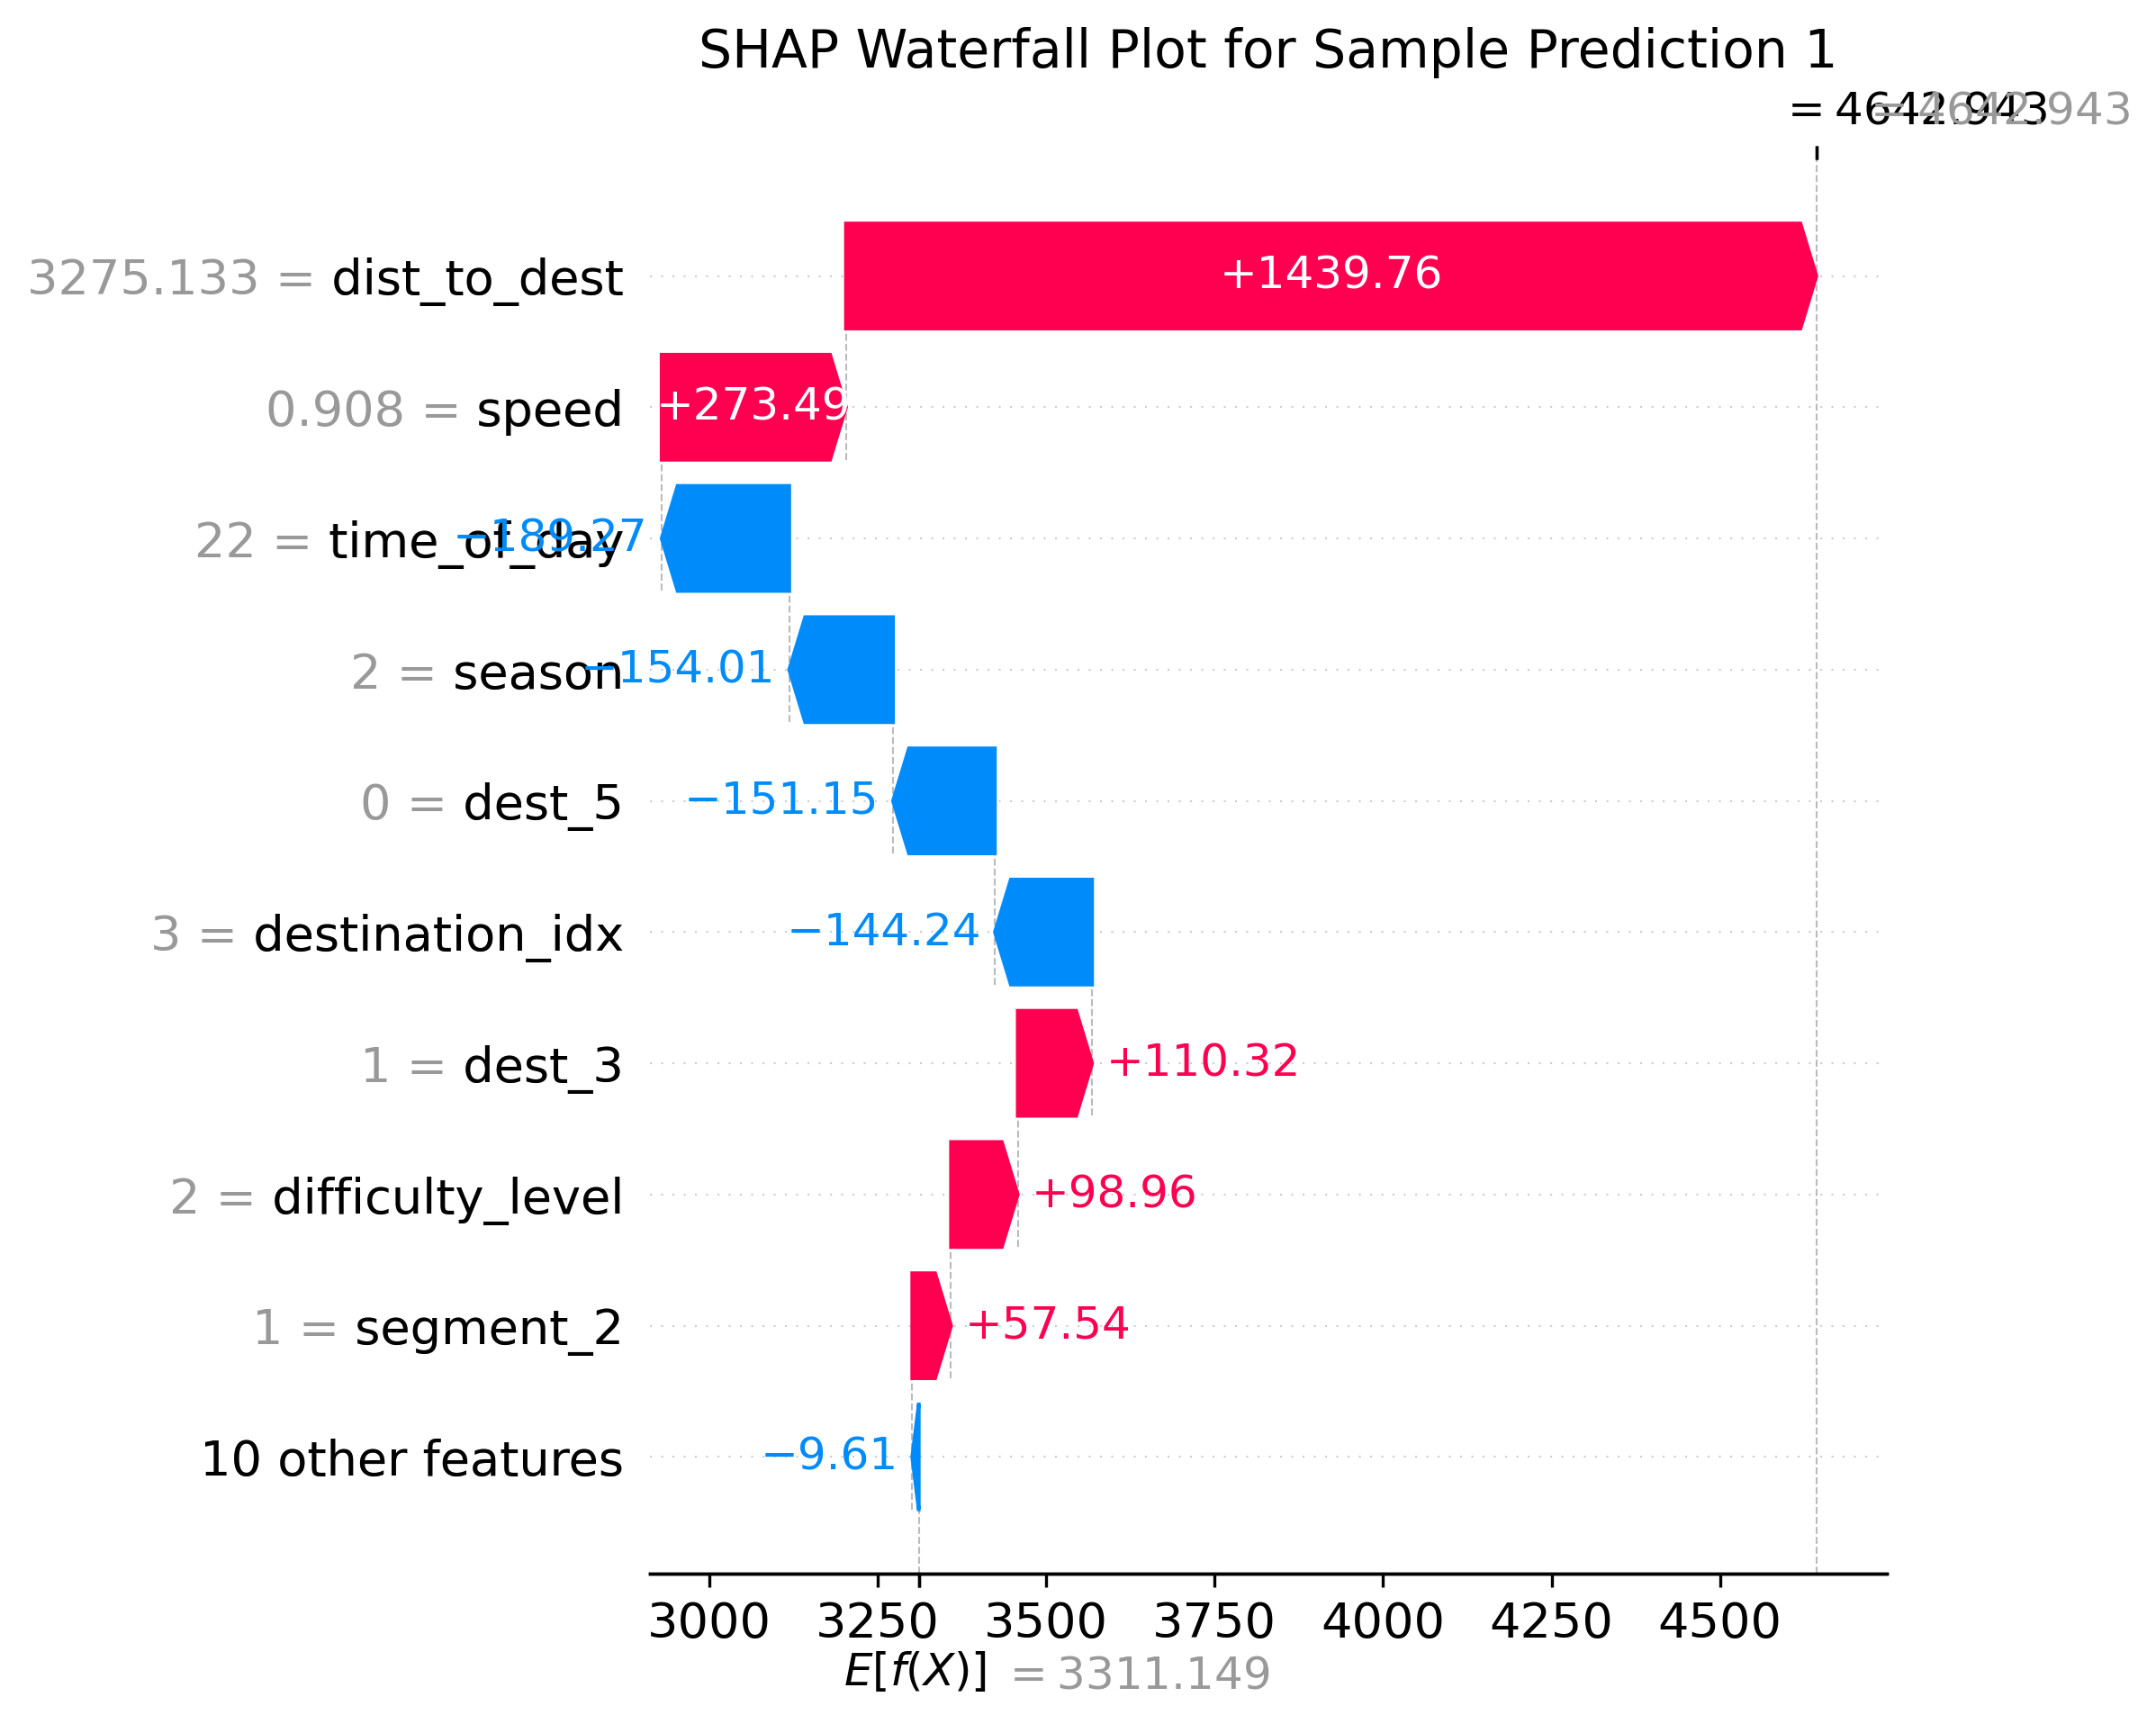
\includegraphics[width=0.9\textwidth]{visualization_results/shap_waterfall_sample_1.png}
\caption{SHAP Waterfall Plot for a Sample Prediction}
\label{fig:shap_waterfall}
\end{figure}

The waterfall plot in Figure \ref{fig:shap_waterfall} demonstrates how individual features contribute to a specific prediction, showing both the magnitude and direction of each feature's impact. This level of interpretability is crucial for understanding why certain predictions might deviate from actual times, especially in the more challenging segments of the route.

\subsection{Single Track Error Analysis}

To gain a deeper understanding of the model's performance on individual tracks, we selected representative tracks for error visualization analysis, as shown in Figures \ref{fig:track_error} and \ref{fig:track_error_dist}:

\begin{figure}[H]
\centering
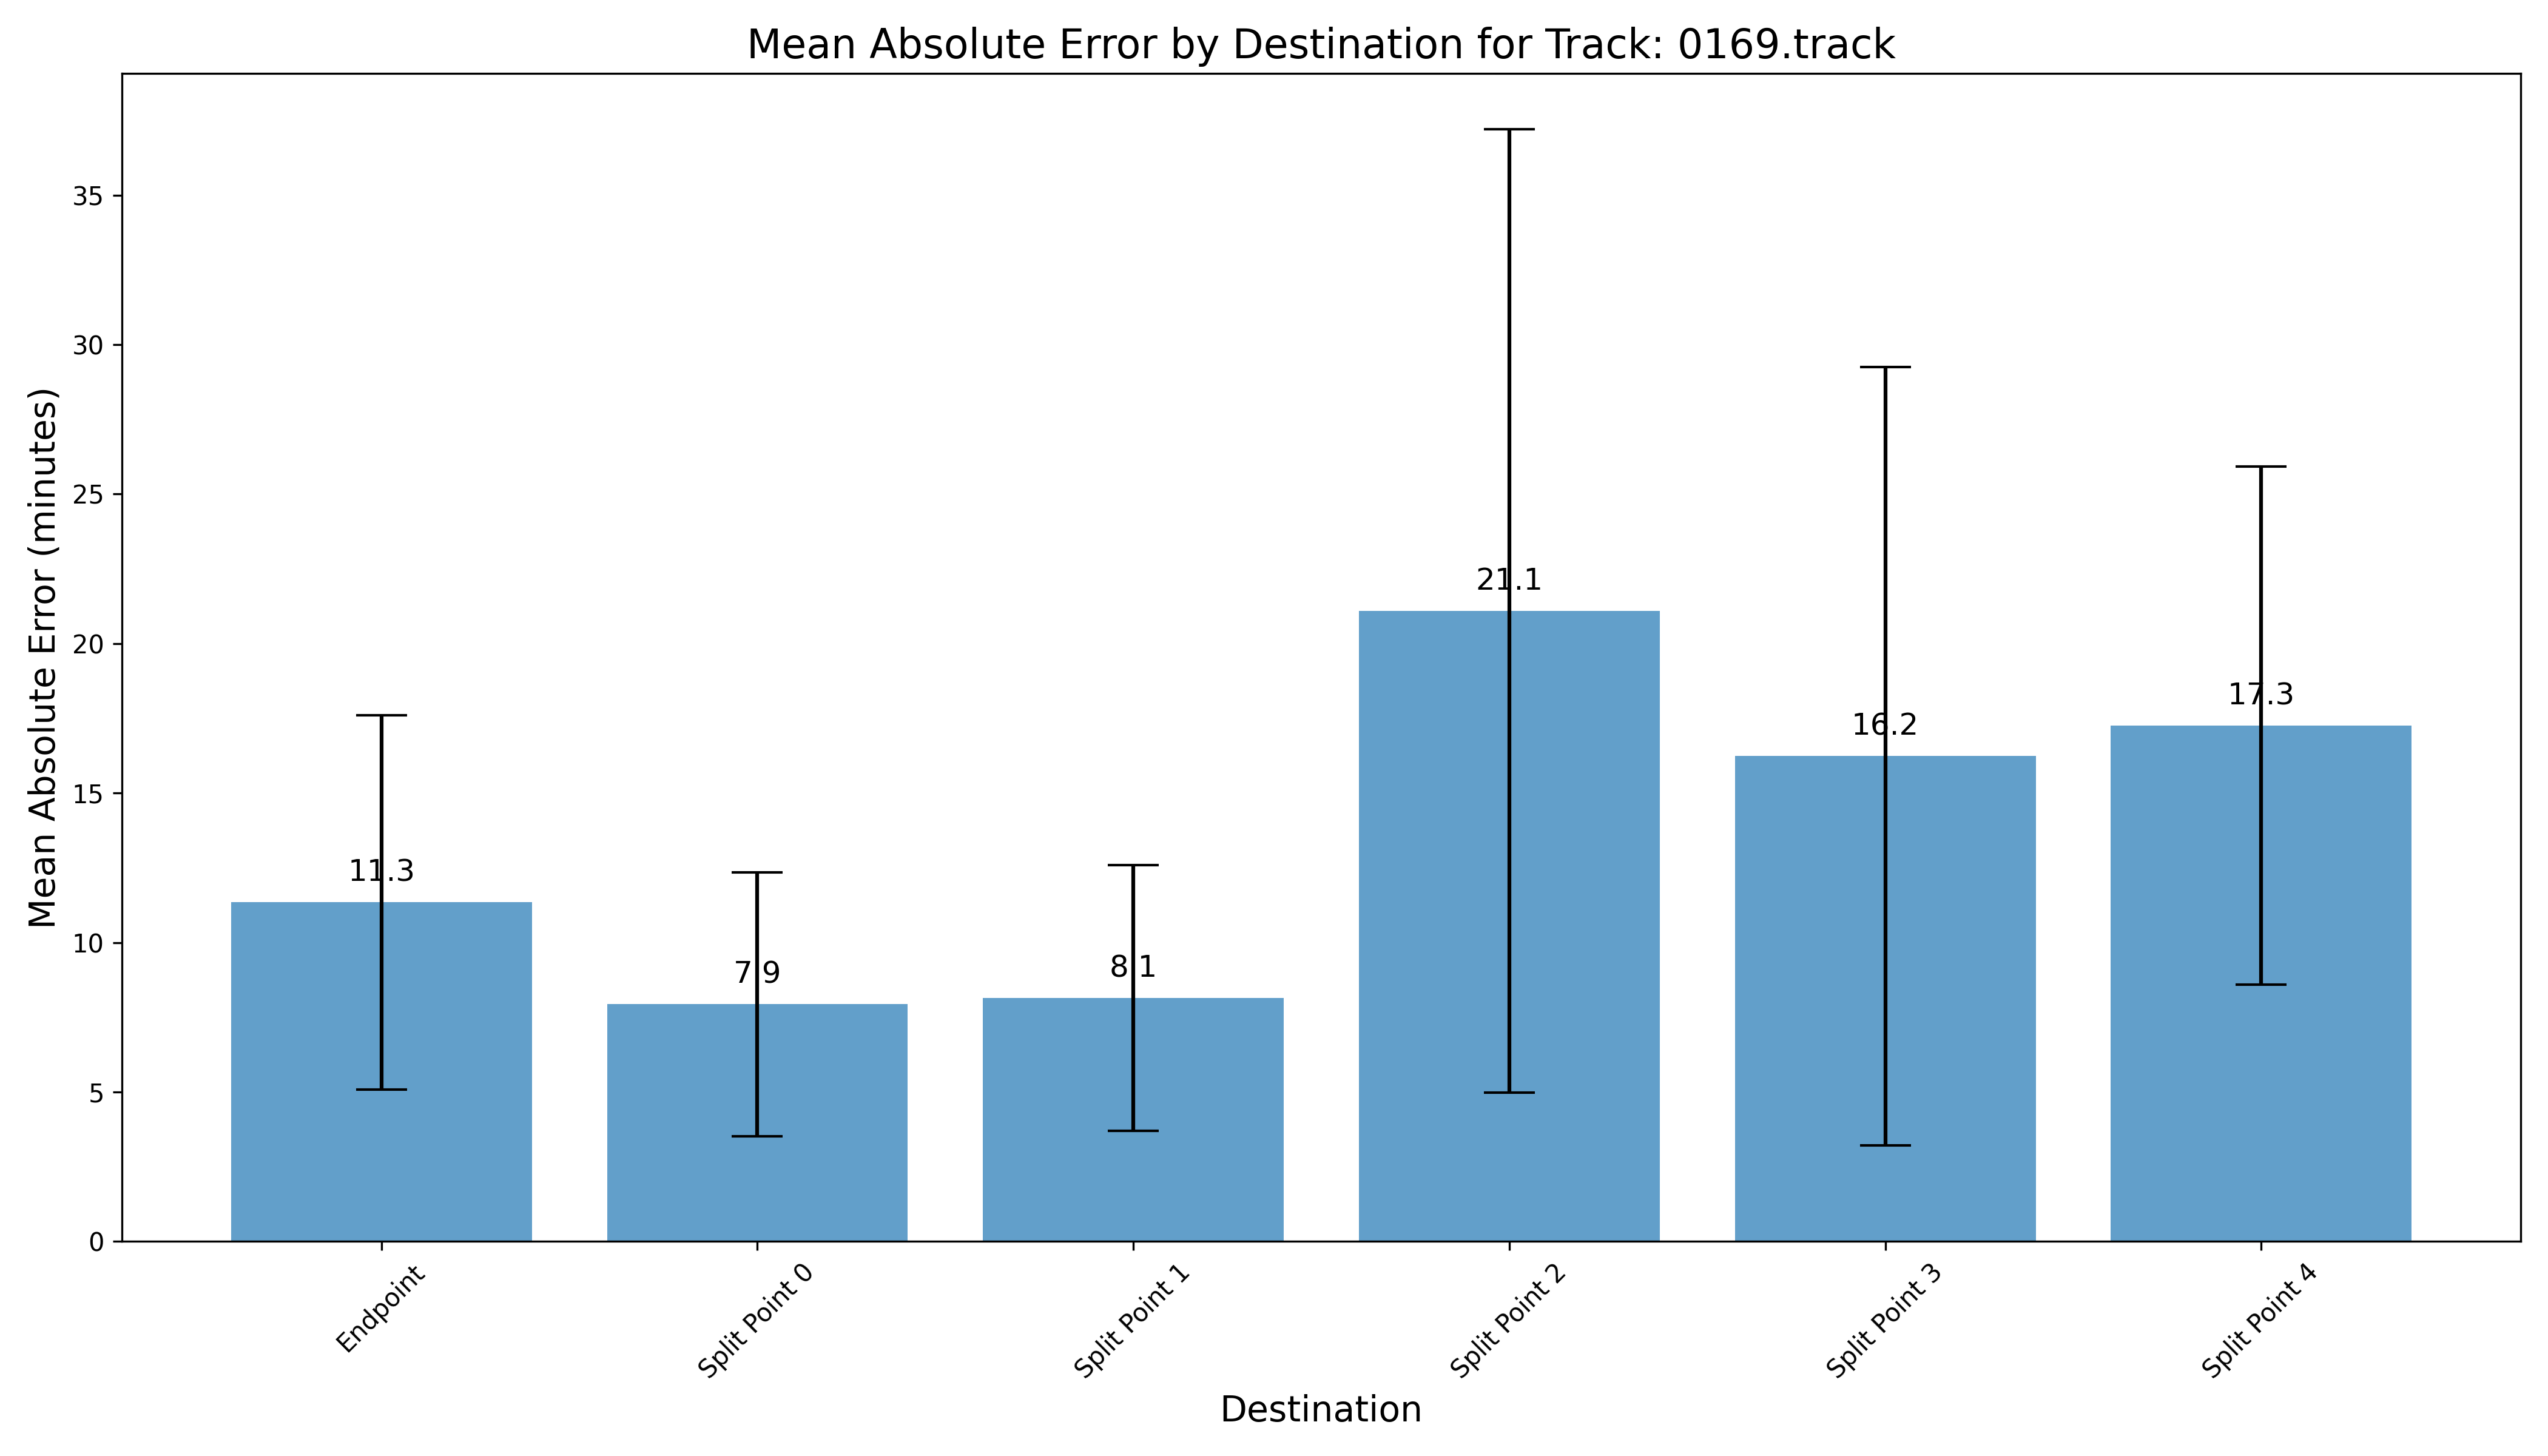
\includegraphics[width=0.8\textwidth]{visualization_results/track_error_by_dest_0169.track.png}
\caption{Single Track Error Analysis Grouped by Destination}
\label{fig:track_error}
\end{figure}

\begin{figure}[H]
\centering
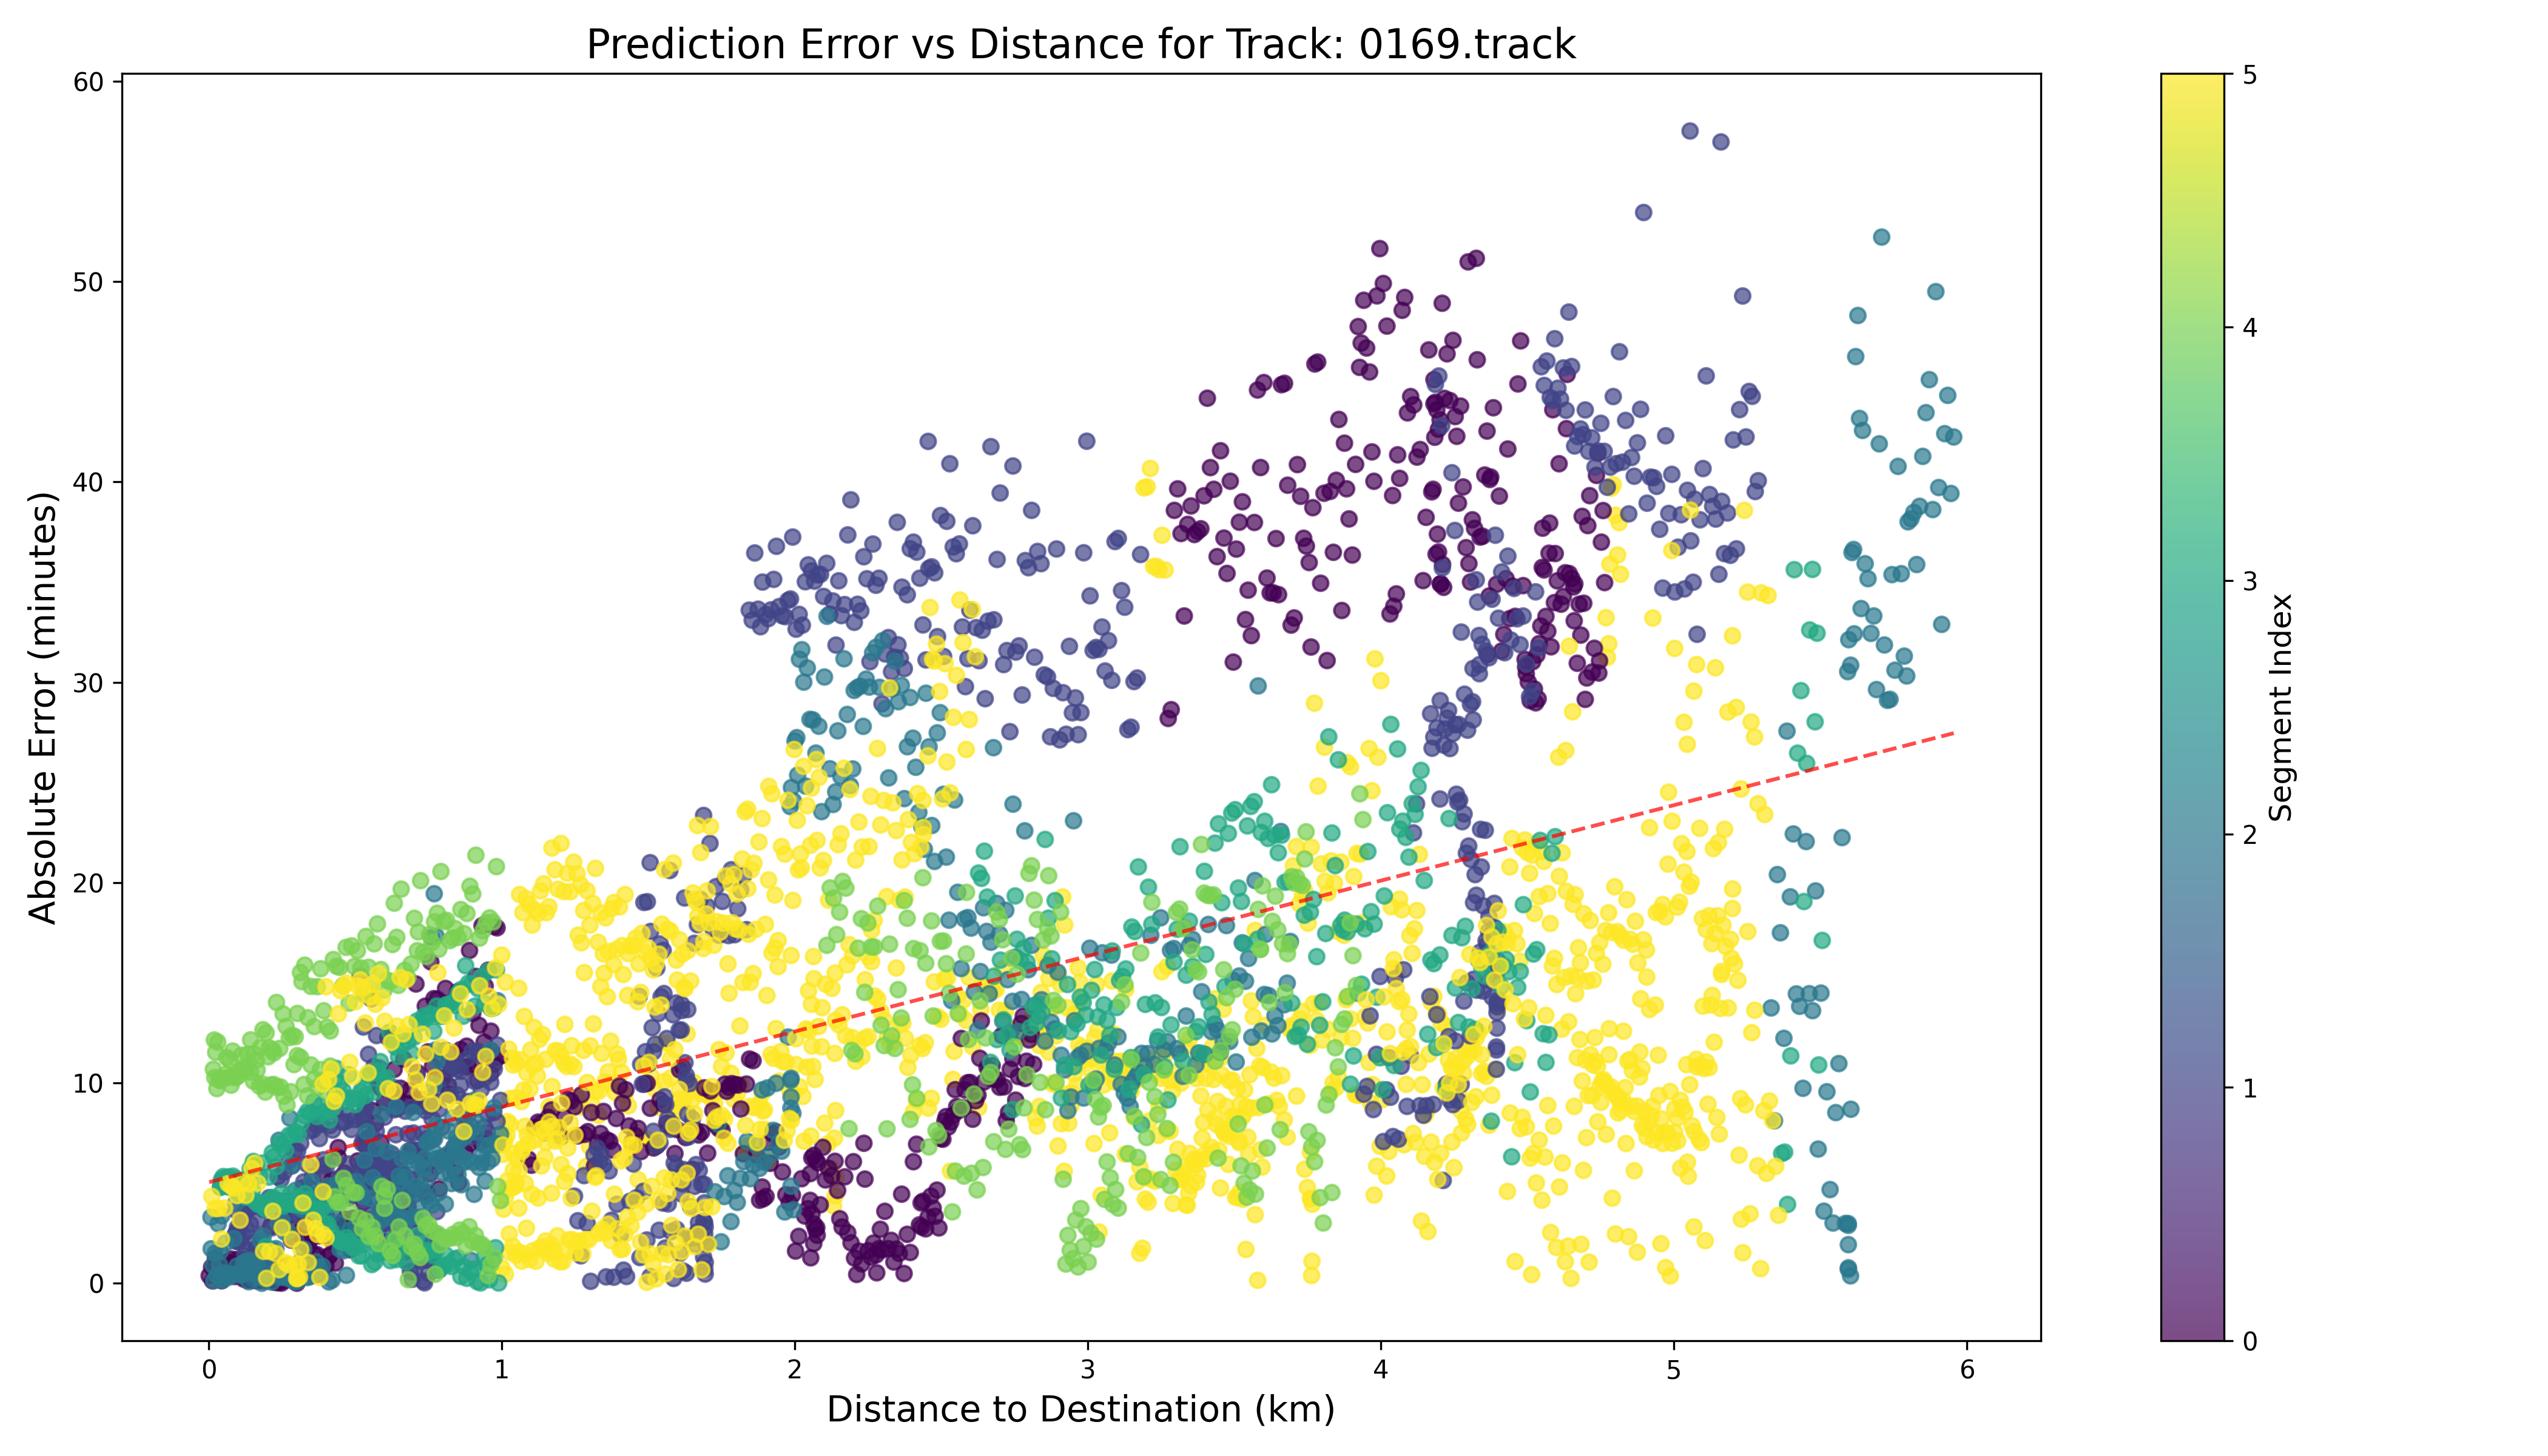
\includegraphics[width=0.8\textwidth]{visualization_results/track_error_vs_distance_0169.track.png}
\caption{Single Track Error vs. Distance Relationship Analysis}
\label{fig:track_error_dist}
\end{figure}

From the single track analysis, we observed the following patterns:

\begin{itemize}
  \item Errors increase with distance, with far-distance predictions usually having larger errors
  \item Prediction errors for different destinations show significant differences
  \item The prediction accuracy for the same track varies across different segments, related to the terrain features of the segment
  \item Certain specific points in the track (such as rest points, steep slopes) may lead to larger prediction errors
\end{itemize}

These findings help us understand the limitations of the model and provide directions for future improvements.

\section{Discussion}

\subsection{Model Performance Analysis}

The XGBoost model built in this study achieved excellent results in predicting Kora time, with an $R^2$ of 0.90 and an average error of only 2.82\%. This result is superior to traditional linear estimation methods based on distance (improvement of about 30.69\%), indicating that machine learning methods have significant advantages in handling journey predictions under complex terrain conditions.

A detailed analysis of model performance across different route segments reveals patterns that directly correlate with the physical characteristics of the terrain:

\begin{itemize}
  \item \textbf{Terrain Complexity and Error Correlation}: The fourth segment (Second Prostration Point to Dazhen Supply Point) has the largest prediction error (380 seconds) despite being only 1.5km long. This segment has the highest difficulty rating (5) due to its undulating terrain. The model's struggle with this segment demonstrates how terrain complexity introduces prediction challenges that go beyond simple distance-based calculations.
  
  \item \textbf{Distance-Difficulty Relationship}: Interestingly, segment 3 (Chuku Temple to Second Prostration Point) is the longest segment (5.5km) with substantial elevation gain (+120m) and has the second-highest error (300 seconds). This suggests a compounding effect where longer distances combined with challenging terrain (difficulty level 4) create greater prediction uncertainty.
  
  \item \textbf{Elevation Profile Impact}: The segments with minimal elevation change (segments 1 and 2 with -50m and +10m respectively) show the lowest prediction errors (100 and 180 seconds). This pattern confirms that the model performs best on segments with consistent elevation profiles, while segments with more variable elevation changes present greater challenges.
  
  \item \textbf{Segment Length vs. Difficulty}: The data reveals a non-intuitive relationship between segment length and prediction difficulty. Segment 2 (2.4km, difficulty 2) has a higher error (180 seconds) than segment 1 (2.3km, difficulty 0), despite similar lengths. This highlights how the model correctly captures the impact of terrain difficulty beyond mere distance.
\end{itemize}

These findings demonstrate that the model's performance characteristics directly reflect the physical reality of the Kora route, with prediction challenges increasing proportionally with terrain complexity rather than simply with distance.

\subsection{Feature Influence Mechanism}

Distance is the most important prediction factor, but the model also captures other important influencing factors:

\begin{itemize}
  \item \textbf{Destination Specificity}: Time predictions for different destinations need to consider their unique features, such as the steep slope before Gangjia Temple.
  \item \textbf{Segment Characteristics}: Certain segments (such as segment\_4) have significant impacts on prediction, indicating that segment characteristics are important considerations.
  \item \textbf{Time Factors}: Although contributing less, time and season do affect travel speed, possibly related to temperature, lighting, and crowd flow.
\end{itemize}

\subsection{Model Comparison: XGBoost vs. Neural Network}

To validate our choice of XGBoost as the primary modeling approach, we conducted a comparative analysis with a feed-forward neural network model. The neural network consisted of three dense layers (64, 32, and 16 neurons) with ReLU activation functions and dropout layers to prevent overfitting.

\begin{figure}[H]
\centering
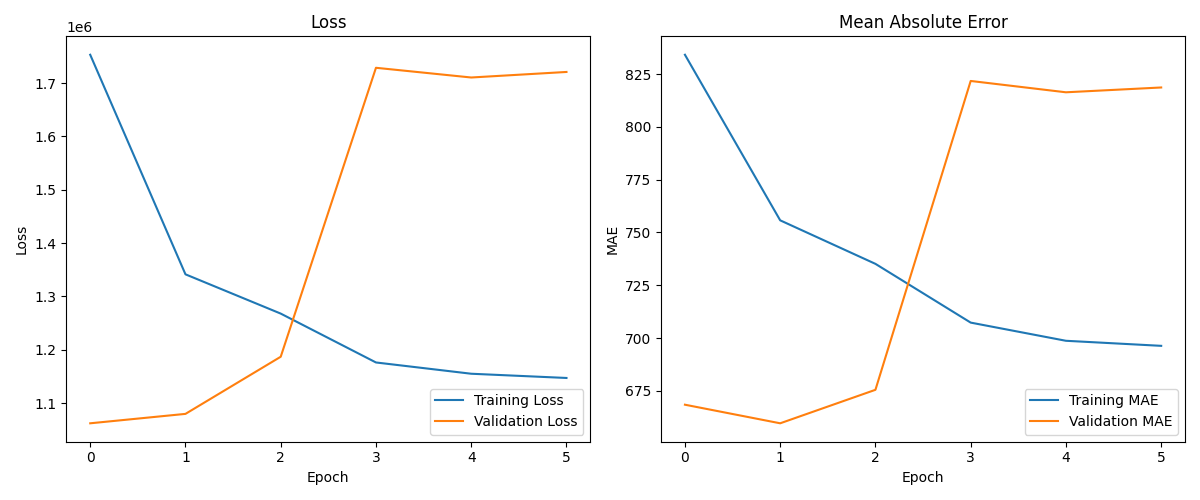
\includegraphics[width=0.8\textwidth]{nn_results/training_history.png}
\caption{Neural Network Training History Showing Loss and MAE Over Epochs}
\label{fig:nn_training}
\end{figure}

Figure \ref{fig:nn_training} shows the training history of the neural network model. While the model successfully converged, it achieved an MAE of 671.26, RMSE of 1040.28, and R² of 0.88. In comparison, our XGBoost model achieved superior performance with lower error metrics and higher explained variance.

\begin{figure}[H]
\centering
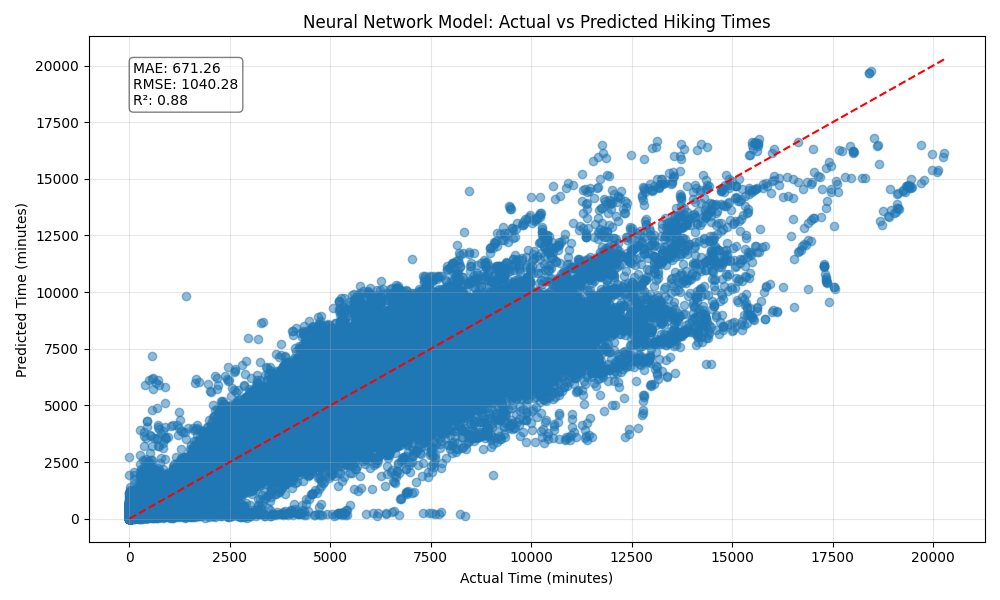
\includegraphics[width=0.8\textwidth]{nn_results/predictions.png}
\caption{Neural Network Model: Actual vs. Predicted Hiking Times}
\label{fig:nn_predictions}
\end{figure}

As shown in Figure \ref{fig:nn_predictions}, the neural network's predictions exhibit greater scatter around the perfect prediction line compared to the XGBoost model, particularly for longer hiking times. This comparison validates our choice of XGBoost for several reasons:

\begin{itemize}
  \item \textbf{Feature-Based Nature}: The hiking time prediction problem is better suited to tree-based models that can capture non-linear relationships between terrain features and hiking times without requiring sequential data structures.
  \item \textbf{Data Efficiency}: XGBoost makes more efficient use of the available data, requiring fewer samples to achieve good generalization.
  \item \textbf{Interpretability}: Unlike neural networks, which function as 'black boxes', XGBoost provides clear feature importance metrics and, as demonstrated through our SHAP analysis, allows for detailed interpretation of how each feature influences predictions.
\end{itemize}

This comparison demonstrates that while deep learning approaches can achieve reasonable performance for hiking time prediction, tree-based ensemble methods like XGBoost are better suited to this particular problem domain, offering both superior accuracy and interpretability.

\subsection{Application Value}

The practical application value of this research is mainly reflected in:

\begin{itemize}
  \item \textbf{Journey Planning}: Helping pilgrims develop reasonable Kora plans, avoiding the risk of not reaching accommodation points before sunset.
  \item \textbf{Safety Assurance}: Providing accurate time estimates, reducing safety hazards in high-altitude environments.
  \item \textbf{Resource Allocation}: Assisting management departments in predicting crowd distribution, reasonably allocating medical and supply resources.
  \item \textbf{Personalized Recommendations}: Providing customized journey recommendations and risk reminders based on individual circumstances.
\end{itemize}

\subsection{Limitations}

Despite the model's good performance, it still has the following limitations:

\begin{itemize}
  \item \textbf{Individual Differences}: Unable to fully consider individual factors such as pilgrims' age, gender, and physical fitness.
  \item \textbf{Environmental Variables}: Lack of real-time data on weather, temperature, snow accumulation, and other environmental factors.
  \item \textbf{Rest Behavior}: Difficult to accurately predict pilgrims' rest frequency and duration, which may lead to increased errors in long-distance predictions.  
\end{itemize}

\section{Conclusion and Future Work}

\subsection{Conclusion}

This paper presents a flexible time prediction model for the Kora route around Mount Kailash. By dividing the route into segments based on terrain characteristics and incorporating features such as distance, gradient, and difficulty level, we achieved a prediction accuracy that significantly outperforms traditional methods.

Our model demonstrates that machine learning approaches can effectively capture the complex relationships between terrain features and hiking times, providing more reliable estimates for pilgrims and trekkers. The segment-based approach allows for more granular predictions that account for the varying difficulty levels along the route.

The SHAP analysis further validates our approach by providing interpretable insights into the model's decision-making process. It reveals that while distance remains a dominant predictor overall, the influence of terrain characteristics varies significantly across different segments. Particularly in challenging segments like segment 4, the difficulty level and gradient features have disproportionate impacts on hiking time predictions. The non-linear relationship between gradient and hiking time, clearly visualized in the SHAP dependence plots, explains why even short segments with steep sections can significantly slow hikers down.

These insights not only improve our understanding of the model but also align with the physical reality of the Kora route, where certain short but challenging sections are known to be particularly time-consuming. The segment-specific SHAP analysis provides a data-driven explanation for this phenomenon, validating both our segmentation approach and the difficulty ratings assigned to each segment.

Future work could explore the integration of additional features such as weather conditions, hiker experience levels, and physiological data to further enhance prediction accuracy. The methodology and interpretability techniques presented here could also be extended to other hiking routes with similar terrain diversity, potentially leading to more accurate and personalized hiking time predictions for various outdoor activities.

\subsection{Future Work}

Based on the findings and limitations of this study, future work can be developed in the following aspects:

\begin{itemize}
  \item \textbf{Model Extension}: Extend the prediction model to the entire Kora route (approximately 52 kilometers), building a complete Kora time prediction system.
  \item \textbf{Personalized Prediction}: Incorporate individual physiological characteristics, health information, and Kora experience to provide personalized time predictions.
  \item \textbf{Dynamic Features}: Introduce dynamic environmental features such as real-time weather, temperature, and snow depth to improve the adaptability of predictions.
  \item \textbf{Advanced Models}: Try deep learning models such as LSTM or Transformer to better capture time series characteristics.
  \item \textbf{Multi-modal Fusion}: Combine satellite images, elevation data, and other multi-source information to enhance the model's understanding of terrain.
  \item \textbf{Real-time System}: Develop a mobile application based on this model to provide pilgrims with real-time journey predictions and safety reminders.
\end{itemize}

This research provides a new methodological reference for time prediction of high-altitude pilgrimage routes, and its technical approach and findings can be extended to other similar scenarios, such as high mountain trekking, outdoor adventure, and other time prediction tasks.

\section{References}

\bibliographystyle{plain}
\begin{thebibliography}{99}

\bibitem{Horiuchi2016}
Horiuchi, M., Endo, J., Akatsuka, S., Uno, T., Hasegawa, T., \& Kikuchi, Y. (2016).
Influence of progressive hypoxia on cardiovascular responses during dynamic exercise in high-altitude residents.
\textit{Journal of Applied Physiology}, 121(1), 139-147.

\bibitem{Ainslie2005}
Ainslie, P. N., Campbell, I. T., Frayn, K. N., Humphreys, S. M., MacLaren, D. P., Reilly, T., \& Westerterp, K. R. (2005).
Energy balance, metabolism, hydration, and performance during strenuous hill walking: the effect of age.
\textit{Journal of Applied Physiology}, 93(2), 714-723.

\end{thebibliography}

\end{document}
